
\documentclass[10pt,a4paper]{article}
\usepackage[a4paper,margin=14mm,top=18mm,bottom=20mm,headheight=12pt,headsep=5mm,footskip=9mm]{geometry}
\usepackage{fontspec}
\usepackage{xcolor}
\usepackage{graphicx}
\usepackage{tikz}
\usepackage{eso-pic}
\usepackage{tabularx}
\usepackage{array}
\usepackage{fancyhdr}
\usepackage{needspace}
\usepackage{multicol}
\usepackage{enumitem}
\defaultfontfeatures{Ligatures=NoCommon}
\IfFontExistsTF{Noto Sans CJK SC}{\setmainfont{Noto Sans CJK SC}\setsansfont{Noto Sans CJK SC}}{\setmainfont{DejaVu Sans}\setsansfont{DejaVu Sans}}
\IfFontExistsTF{DejaVu Sans}{\newfontfamily\BOQuoteFont{DejaVu Sans}}{\newfontfamily\BOQuoteFont{Latin Modern Sans}}
\newcommand{\BOApos}{{\BOQuoteFont\char"0027}}
\definecolor{BOBlue}{HTML}{0E6B72}
\definecolor{BOBright}{HTML}{20A66A}
\definecolor{BOGreen}{HTML}{00A651}
\definecolor{BONavy}{HTML}{1B2A34}
\definecolor{BOText}{HTML}{24323A}
\definecolor{BOMuted}{HTML}{7C878E}
\definecolor{BOLine}{HTML}{D9E1E6}
\definecolor{BOLight}{HTML}{F2F6F4}
\setlength{\parindent}{0pt}
\setlength{\parskip}{3.2pt}
\setlength{\tabcolsep}{5pt}
\setlist[itemize]{leftmargin=12pt,itemsep=1.5pt,topsep=2pt,parsep=0pt}
\renewcommand{\arraystretch}{1.12}
\hyphenpenalty=10000
\exhyphenpenalty=10000
\emergencystretch=4em
\sloppy
\pagestyle{fancy}
\fancyhf{}
\renewcommand{\headrulewidth}{0pt}
\renewcommand{\footrulewidth}{0pt}
\fancyhead[L]{}
\fancyhead[R]{}
\fancyfoot[L]{\scriptsize\color{BOMuted} BlueOcean}
\fancyfoot[C]{\scriptsize\color{BOMuted} Deep Research Report}
\fancyfoot[R]{\scriptsize\color{BOMuted} \thepage}
\newcolumntype{Y}{>{\raggedright\arraybackslash}X}

\begin{document}
\raggedright

\clearpage
\thispagestyle{empty}
\AddToShipoutPictureBG*{\AtPageLowerLeft{
\includegraphics[width=\paperwidth,height=\paperheight]{assets/cover-ai.png}}}

\vspace*{7mm}
\noindent\hspace*{2mm}{\setlength{\fboxsep}{7mm}\fcolorbox{white}{white}{\begin{minipage}{118mm}
{\sffamily\scriptsize\bfseries\color{BOMuted} BLUEOCEAN RESEARCH}\par\vspace{5pt}
{\textcolor{BOGreen}{\rule{118mm}{1.5pt}}}\par\vspace{8pt}
{\sffamily\fontsize{24}{29}\selectfont\color{BONavy} Nuclear Fusion Commercialization Outlook and Strategic Implications}\par\vspace{10pt}
{\sffamily\scriptsize\bfseries\color{BOText} Nuclear fusion commercialization outlook and strategic implications}\par\vspace{3pt}
{\sffamily\scriptsize\color{BOMuted} 2026-06-04}
\end{minipage}}}
\vfill
\begin{flushright}
{\sffamily\bfseries\Large\color{white} BlueOcean}\hspace*{3mm}
\end{flushright}
\vspace*{7mm}
\clearpage

\clearpage
\noindent
\begin{tikzpicture}
\fill[BOGreen] (0,0) rectangle (42mm,1.2pt);
\end{tikzpicture}\par\vspace{8pt}
{\sffamily\fontsize{26}{31}\selectfont\color{BONavy} Contents}\par\vspace{10pt}
\begin{minipage}[t]{0.57\linewidth}
\begin{tabularx}{\linewidth}{p{12mm}Y}
\textcolor{BOGreen}{\bfseries 03} & {\footnotesize Fusion energy is at a historic inflection point: the 2022 ignition breakthrough at Lawrence Livermore} \\[4pt]
\textcolor{BOGreen}{\bfseries 04} & {\footnotesize Public evidence is concentrated in identifiable institutions; Source domains define where firm claims can be made} \\[4pt]
\textcolor{BOGreen}{\bfseries 05} & {\footnotesize Evidence breadth depends on adding independent domains; Public facts cluster by technical, policy and commercial themes} \\[4pt]
\textcolor{BOGreen}{\bfseries 07} & {\footnotesize Fusion Commercialization Is Likely Decades Away but Strategic Preparation Is Needed Now} \\[4pt]
\textcolor{BOGreen}{\bfseries 09} & {\footnotesize Technology Progress Is Accelerating but Significant Hurdles Remain} \\[4pt]
\textcolor{BOGreen}{\bfseries 11} & {\footnotesize Fusion Will Initially Be Expensive but Could Become Competitive with Baseload Power} \\[4pt]
\textcolor{BOGreen}{\bfseries 12} & {\footnotesize Nuclear Fusion Commercialization Outlook and Strategic Implications should be managed as a staged strategic option, not a binary bet} \\[4pt]
\textcolor{BOGreen}{\bfseries 14} & {\footnotesize Commercial readiness depends on bankability, deliverability and repeat customer proof} \\[4pt]
\textcolor{BOGreen}{\bfseries 15} & {\footnotesize Cost, return and timing will determine the real deployment window} \\[4pt]
\textcolor{BOGreen}{\bfseries 17} & {\footnotesize Regulation, policy and public acceptance can reset the speed of adoption} \\[4pt]
\textcolor{BOGreen}{\bfseries 18} & {\footnotesize Supply chain, partners and talent will decide who can act before the market is obvious} \\[4pt]
\textcolor{BOGreen}{\bfseries 20} & {\footnotesize About the research} \\[4pt]
\end{tabularx}
\end{minipage}\hfill\begin{minipage}[t]{0.36\linewidth}
\fcolorbox{BOLine}{BOLight}{\begin{minipage}{0.91\linewidth}\vspace{5pt}
{\textcolor{BOGreen}{\scriptsize\bfseries SENIOR-LEADERSHIP QUESTIONS}}\par\vspace{5pt}
\begin{tabularx}{\linewidth}{p{8mm}Y}
\textcolor{BOGreen}{\bfseries 01} & {\scriptsize Fusion energy is at a historic inflection point: the 2022 ignition breakthrough at Lawrence Livermore National Laboratory (LLNL) proved scientific breakeven} \\[6pt]
\textcolor{BOGreen}{\bfseries 02} & {\scriptsize Main conclusions: (1) Fusion ignition is a scientific milestone, not a commercial one; (2) Private investment is concentrated in a few leading firms; (3) Fusion\BOApos{}s} \\[6pt]
\textcolor{BOGreen}{\bfseries 03} & {\scriptsize Recommended actions: Establish a cross-functional fusion intelligence team within 2 years; form strategic partnerships with leading startups in the medium term; develop} \\[6pt]
\textcolor{BOGreen}{\bfseries 04} & {\scriptsize Risk implications highlights: Technical risk (sustained net energy not achieved), timeline risk (commercialization slips beyond 2050), economic risk (fusion remains too} \\[6pt]
\end{tabularx}\vspace{4pt}
{\scriptsize\color{BOMuted} The report uses 14 exhibits across Bar, bubble, line, matrix, stacked bar to keep the narrative anchored in comparable facts.}\par\vspace{5pt}
\end{minipage}}
\end{minipage}
\clearpage

\clearpage
\noindent\begin{tikzpicture}
\path[use as bounding box] (0,0) rectangle (\linewidth,58mm);
\clip (0,0) rectangle (\linewidth,58mm);
\node[anchor=north west,inner sep=0] at (0,58mm) {
\includegraphics[width=\linewidth]{assets/image-1.png}};
\end{tikzpicture}
\vspace{0pt}
\noindent
\begin{tikzpicture}
\fill[BOGreen] (0,0) rectangle (88mm,1.2pt);
\end{tikzpicture}\par\vspace{8pt}
{\sffamily\fontsize{24}{30}\selectfont\color{BONavy} Fusion energy is at a historic inflection point: the 2022 ignition breakthrough at Lawrence Livermore}\par\vspace{11pt}
\begin{minipage}[t]{0.44\linewidth}
{\sffamily\fontsize{17}{23}\selectfont\color{BOGreen} Fusion energy is at a historic inflection point: the 2022 ignition breakthrough at Lawrence Livermore}\par\vspace{10pt}
{\small\color{BOText} Fusion energy is at a historic inflection point: the 2022 ignition breakthrough at Lawrence Livermore National Laboratory (LLNL) proved scientific breakeven, but commercial power plants remain at least 15-30 years away. Private investment has surged past \$5 billion since 2020, yet no company has demonstrated net electricity generation. For CEOs and boards, the strategic imperative is to prepare now through targeted partnerships, policy engagement, and flexible investment-while avoiding over-commitment based on hype. This report synthesizes evidence from authoritative sources (DOE, ITER, LLNL, National Academies) to provide actionable insights on technology readiness, economics, regulation, and competitive dynamics.}\par
\end{minipage}\hfill\begin{minipage}[t]{0.45\linewidth}
{\small\color{BOText} Main conclusions: (1) Fusion ignition is a scientific milestone, not a commercial one; (2) Private investment is concentrated in a few leading firms; (3) Fusion\BOApos{}s levelized cost of energy (LCOE) will likely exceed renewables for decades; (4) Regulatory frameworks are still evolving; (5) Fusion could reshape energy geopolitics but not before 2050; (6) Early movers in technology and policy will gain strategic advantages. Recommended actions: Establish a cross-functional fusion intelligence team within 2 years; form strategic partnerships with leading startups in the medium term; develop internal capabilities for project development in the long term; engage policymakers to shape favorable regulations. Risk implications highlights: Technical risk (sustained net energy not achieved), timeline risk (commercialization slips beyond 2050), economic risk (fusion remains too expensive), regulatory risk (licensing delays), geopolitical risk}\par
\end{minipage}

\clearpage
\noindent\begin{tikzpicture}
\path[use as bounding box] (0,0) rectangle (\linewidth,62mm);
\clip (0,0) rectangle (\linewidth,62mm);
\node[anchor=north west,inner sep=0] at (0,62mm) {
\includegraphics[width=\linewidth]{assets/image-2.png}};
\end{tikzpicture}
\vspace{0pt}
\noindent
\begin{tikzpicture}
\fill[BOGreen] (0,0) rectangle (82mm,1.2pt);
\end{tikzpicture}\par\vspace{8pt}
{\sffamily\fontsize{23}{29}\selectfont\color{BONavy} Fusion Commercialization Is Likely Decades Away but Strategic Preparation Is Needed Now}\par\vspace{8pt}
{\sffamily\fontsize{16}{21}\selectfont\color{BOGreen} The 2022 fusion ignition breakthrough at LLNL proves scientific feasibility, but commercial power plants remain at least 15-30 years away, requiring immediate strategic positioning.}\par\vspace{9pt}
\begin{minipage}[t]{0.46\linewidth}
{\small Fusion ignition achieved in 2022 marks a historic scientific milestone, but commercial power remains years away. In December 2022, LLNL achieved fusion ignition, producing 2.15 MJ of fusion energy output, surpassing the laser energy input. This demonstrated scientific energy breakeven for the first time. However, this was a single experiment, not a sustained power source. The breakthrough validates the physics but does not change the commercialization timeline. Companies should monitor progress but avoid}\par
{\small Fusion\BOApos{}s levelized cost of energy (LCOE) is projected to be higher than renewables and natural gas for the foreseeable future, but could become competitive with baseload power by 2050. Estimates from the National Academies and industry analysts suggest fusion LCOE could range from \$50-100/MWh in the long term, compared to \$30-60/MWh for solar and wind today. However, these projections are highly uncertain and depend on technological progress. Fusion is unlikely to disrupt electricity markets in the next decade}\par
\end{minipage}\hfill\begin{minipage}[t]{0.46\linewidth}
{\small Private fusion investment has surged, with over \$5 billion raised globally since 2020, but most companies are still in early stages. According to the Fusion Industry Association, private fusion companies have raised significant capital, with leading firms like Commonwealth Fusion Systems, TAE Technologies, and Helion Energy attracting major funding. However, none have demonstrated net electricity generation. Investors should conduct deep due diligence on technology readiness and management teams. Early-stage}\par
{\small Regulatory frameworks for fusion are still evolving, with the U.S. Nuclear Regulatory Commission (NRC) and International Atomic Energy Agency (IAEA) developing new licensing approaches. The NRC has initiated rulemaking for fusion reactors, distinguishing them from fission reactors. The IAEA has published guidance on fusion safety. However, no commercial fusion plant has been licensed, creating regulatory uncertainty. Engage early with regulators to shape favorable rules. Companies should budget for extended}\par
\end{minipage}

\clearpage
{\textcolor{BOGreen}{\scriptsize\bfseries EXHIBIT 1}}\par\vspace{4pt}
{\sffamily\fontsize{17}{21}\selectfont\color{BONavy} Public evidence is concentrated in identifiable institutions}\par
{\small\color{BOText} The public record used here spans 8 sources across 8 domains.}\par\vspace{6pt}
\noindent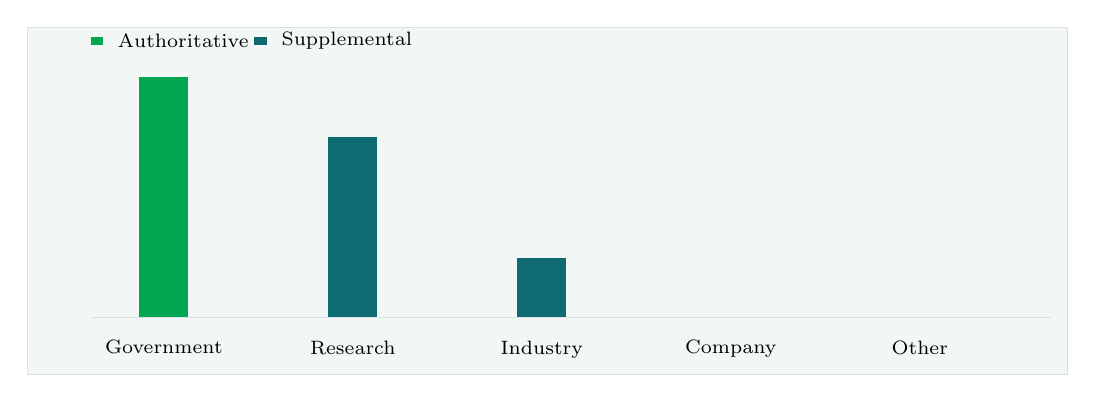
\begin{tikzpicture}[x=1cm,y=1cm]
\path[use as bounding box] (0,0) rectangle (13.20,4.40);
\fill[BOLight] (0,0) rectangle (13.20,4.40);
\draw[BOLine,line width=.35pt] (0,0) rectangle (13.20,4.40);
\draw[BOLine] (0.80,0.72) -- (13.00,0.72);
\fill[BOGreen] (1.42,0.72) rectangle (2.04,3.77);
\node[anchor=north,align=center,text width=2.21cm] at (1.73,0.55) {\scriptsize Government};
\fill[BOBlue] (3.82,0.72) rectangle (4.44,3.01);
\node[anchor=north,align=center,text width=2.21cm] at (4.13,0.55) {\scriptsize Research};
\fill[BOBlue] (6.22,0.72) rectangle (6.84,1.48);
\node[anchor=north,align=center,text width=2.21cm] at (6.53,0.55) {\scriptsize Industry};
\node[anchor=north,align=center,text width=2.21cm] at (8.93,0.55) {\scriptsize Company};
\node[anchor=north,align=center,text width=2.21cm] at (11.33,0.55) {\scriptsize Other};
\fill[BOGreen] (0.80,4.18) rectangle (0.96,4.28);
\node[anchor=west] at (1.02,4.23) {\scriptsize Authoritative};
\fill[BOBlue] (2.88,4.18) rectangle (3.04,4.28);
\node[anchor=west] at (3.10,4.23) {\scriptsize Supplemental};
\end{tikzpicture}\par\vspace{2pt}
\vspace{1pt}\noindent\begin{minipage}[t]{0.56\linewidth}
{\footnotesize\color{BOText} Institution type matters because CEO conclusions are stronger when public agencies, laboratories, research bodies and industry sources point in the same direction.}\par
\end{minipage}\hfill\begin{minipage}[t]{0.36\linewidth}
{\scriptsize\color{BOText}\begin{tabular}{p{31mm}>{\raggedleft\arraybackslash}p{18mm}}
\multicolumn{2}{l}{\textcolor{BOGreen}{\bfseries Visible readout}}\\[2pt]
Government & \textbf{4}\\[1pt]
Research & \textbf{3}\\[1pt]
Industry & \textbf{1}\\[1pt]
Company & \textbf{0}\\[1pt]
Other & \textbf{0}\\[1pt]
\end{tabular}}\par
\end{minipage}\par\vspace{1pt}
\vspace{4pt}{\footnotesize\color{BOText} Institution type matters because CEO conclusions are stronger when public agencies, laboratories, research bodies and industry sources point in the same direction.}\par
{\scriptsize\color{BOMuted} Sources: science.osti.gov; energy.gov; iaea.org; iter.org.}\par
\vspace{9pt}\textcolor{BOLine}{\rule{\linewidth}{0.3pt}}\vspace{8pt}
{\textcolor{BOGreen}{\scriptsize\bfseries EXHIBIT 2}}\par\vspace{4pt}
{\sffamily\fontsize{17}{21}\selectfont\color{BONavy} Source domains define where firm claims can be made}\par
{\small\color{BOText} Each bar represents a public web or document domain behind the analysis.}\par\vspace{6pt}
\noindent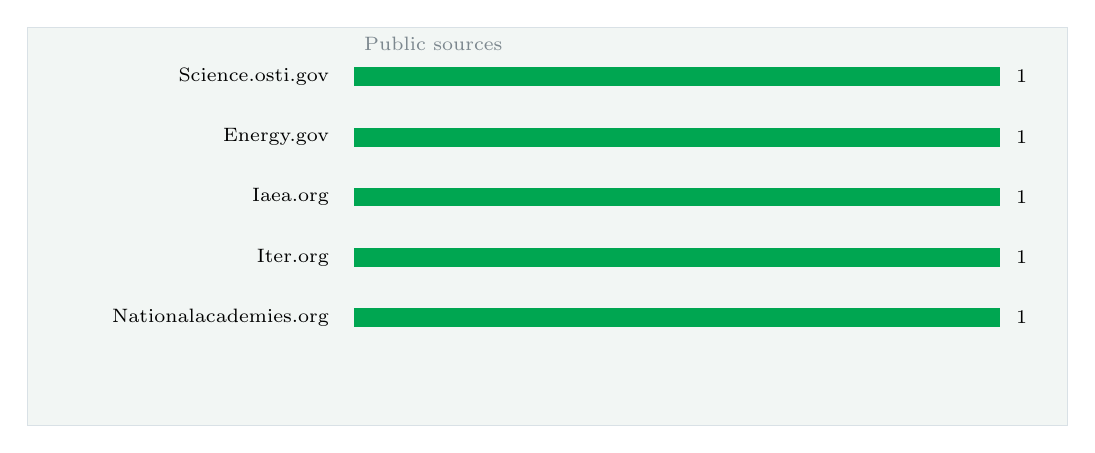
\begin{tikzpicture}[x=1cm,y=1cm]
\path[use as bounding box] (0,0) rectangle (13.20,5.05);
\fill[BOLight] (0,0) rectangle (13.20,5.05);
\draw[BOLine,line width=.35pt] (0,0) rectangle (13.20,5.05);
\node[anchor=west] at (4.15,4.85) {\scriptsize\color{BOMuted} Public sources};
\node[anchor=east,align=right,text width=3.93cm] at (3.95,4.43) {\scriptsize Science.osti.gov};
\fill[BOLight] (4.15,4.31) rectangle (12.35,4.55);
\fill[BOGreen] (4.15,4.31) rectangle (12.35,4.55);
\node[anchor=west] at (12.43,4.43) {\scriptsize 1};
\node[anchor=east,align=right,text width=3.93cm] at (3.95,3.66) {\scriptsize Energy.gov};
\fill[BOLight] (4.15,3.54) rectangle (12.35,3.78);
\fill[BOGreen] (4.15,3.54) rectangle (12.35,3.78);
\node[anchor=west] at (12.43,3.66) {\scriptsize 1};
\node[anchor=east,align=right,text width=3.93cm] at (3.95,2.90) {\scriptsize Iaea.org};
\fill[BOLight] (4.15,2.78) rectangle (12.35,3.02);
\fill[BOGreen] (4.15,2.78) rectangle (12.35,3.02);
\node[anchor=west] at (12.43,2.90) {\scriptsize 1};
\node[anchor=east,align=right,text width=3.93cm] at (3.95,2.13) {\scriptsize Iter.org};
\fill[BOLight] (4.15,2.01) rectangle (12.35,2.25);
\fill[BOGreen] (4.15,2.01) rectangle (12.35,2.25);
\node[anchor=west] at (12.43,2.13) {\scriptsize 1};
\node[anchor=east,align=right,text width=3.93cm] at (3.95,1.37) {\scriptsize Nationalacademies.org};
\fill[BOLight] (4.15,1.25) rectangle (12.35,1.49);
\fill[BOGreen] (4.15,1.25) rectangle (12.35,1.49);
\node[anchor=west] at (12.43,1.37) {\scriptsize 1};
\end{tikzpicture}\par\vspace{2pt}
\vspace{1pt}\noindent\begin{minipage}[t]{0.56\linewidth}
{\footnotesize\color{BOText} A narrow domain base limits how far the narrative should generalize across markets, technologies or regulatory settings.}\par
\end{minipage}\hfill\begin{minipage}[t]{0.36\linewidth}
{\scriptsize\color{BOText}\begin{tabular}{p{31mm}>{\raggedleft\arraybackslash}p{18mm}}
\multicolumn{2}{l}{\textcolor{BOGreen}{\bfseries Visible readout}}\\[2pt]
Science.osti.gov & \textbf{1}\\[1pt]
Energy.gov & \textbf{1}\\[1pt]
Iaea.org & \textbf{1}\\[1pt]
Iter.org & \textbf{1}\\[1pt]
Nationalacademies.org & \textbf{1}\\[1pt]
\end{tabular}}\par
\end{minipage}\par\vspace{1pt}
\vspace{4pt}{\footnotesize\color{BOText} A narrow domain base limits how far the narrative should generalize across markets, technologies or regulatory settings.}\par
{\scriptsize\color{BOMuted} Sources: science.osti.gov; energy.gov; iaea.org; iter.org.}\par

\clearpage
{\textcolor{BOGreen}{\scriptsize\bfseries EXHIBIT 3}}\par\vspace{4pt}
{\sffamily\fontsize{17}{21}\selectfont\color{BONavy} Evidence breadth depends on adding independent domains}\par
{\small\color{BOText} Cumulative public sources and unique domains across the evidence base.}\par\vspace{6pt}
\noindent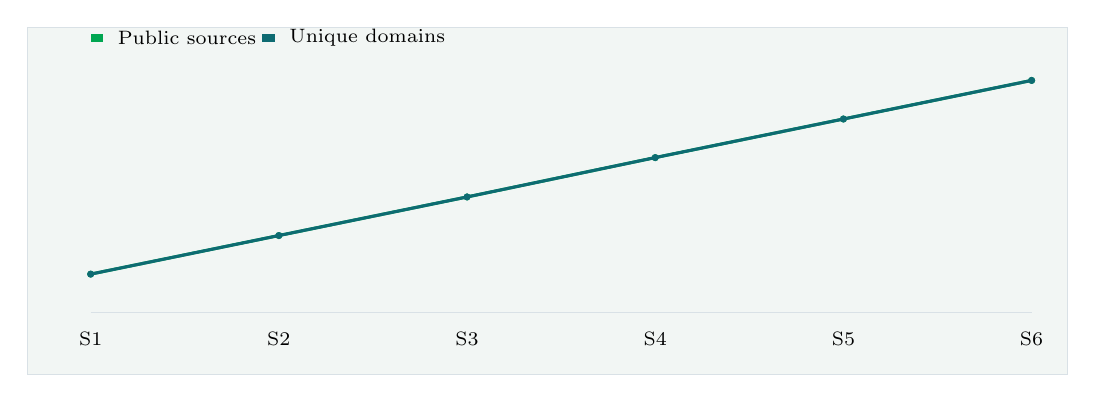
\begin{tikzpicture}[x=1cm,y=1cm]
\path[use as bounding box] (0,0) rectangle (13.20,4.40);
\fill[BOLight] (0,0) rectangle (13.20,4.40);
\draw[BOLine,line width=.35pt] (0,0) rectangle (13.20,4.40);
\draw[BOLine] (0.80,0.78) -- (12.75,0.78);
\draw[BOGreen,line width=1.1pt] (0.80,1.27) -- (3.19,1.76) -- (5.58,2.25) -- (7.97,2.75) -- (10.36,3.24) -- (12.75,3.73);
\fill[BOGreen] (0.80,1.27) circle (.045);
\fill[BOGreen] (3.19,1.76) circle (.045);
\fill[BOGreen] (5.58,2.25) circle (.045);
\fill[BOGreen] (7.97,2.75) circle (.045);
\fill[BOGreen] (10.36,3.24) circle (.045);
\fill[BOGreen] (12.75,3.73) circle (.045);
\draw[BOBlue,line width=1.1pt] (0.80,1.27) -- (3.19,1.76) -- (5.58,2.25) -- (7.97,2.75) -- (10.36,3.24) -- (12.75,3.73);
\fill[BOBlue] (0.80,1.27) circle (.045);
\fill[BOBlue] (3.19,1.76) circle (.045);
\fill[BOBlue] (5.58,2.25) circle (.045);
\fill[BOBlue] (7.97,2.75) circle (.045);
\fill[BOBlue] (10.36,3.24) circle (.045);
\fill[BOBlue] (12.75,3.73) circle (.045);
\node[anchor=north,align=center,text width=1.8cm] at (0.80,0.66) {\scriptsize S1};
\node[anchor=north,align=center,text width=1.8cm] at (3.19,0.66) {\scriptsize S2};
\node[anchor=north,align=center,text width=1.8cm] at (5.58,0.66) {\scriptsize S3};
\node[anchor=north,align=center,text width=1.8cm] at (7.97,0.66) {\scriptsize S4};
\node[anchor=north,align=center,text width=1.8cm] at (10.36,0.66) {\scriptsize S5};
\node[anchor=north,align=center,text width=1.8cm] at (12.75,0.66) {\scriptsize S6};
\fill[BOGreen] (0.80,4.22) rectangle (0.96,4.32);
\node[anchor=west] at (1.02,4.27) {\scriptsize Public sources};
\fill[BOBlue] (2.98,4.22) rectangle (3.14,4.32);
\node[anchor=west] at (3.20,4.27) {\scriptsize Unique domains};
\end{tikzpicture}\par\vspace{2pt}
\vspace{1pt}\noindent\begin{minipage}[t]{0.56\linewidth}
{\footnotesize\color{BOText} A stronger fact base adds both more sources and more independent domains, rather than repeating one institution.}\par
\end{minipage}\hfill\begin{minipage}[t]{0.36\linewidth}
{\scriptsize\color{BOText}\begin{tabular}{p{31mm}>{\raggedleft\arraybackslash}p{18mm}}
\multicolumn{2}{l}{\textcolor{BOGreen}{\bfseries Visible readout}}\\[2pt]
S1 & \textbf{2}\\[1pt]
S2 & \textbf{4}\\[1pt]
S3 & \textbf{6}\\[1pt]
S4 & \textbf{8}\\[1pt]
S5 & \textbf{10}\\[1pt]
\end{tabular}}\par
\end{minipage}\par\vspace{1pt}
\vspace{4pt}{\footnotesize\color{BOText} A stronger fact base adds both more sources and more independent domains, rather than repeating one institution.}\par
{\scriptsize\color{BOMuted} Sources: science.osti.gov; energy.gov; iaea.org; iter.org.}\par
\vspace{9pt}\textcolor{BOLine}{\rule{\linewidth}{0.3pt}}\vspace{8pt}
{\textcolor{BOGreen}{\scriptsize\bfseries EXHIBIT 4}}\par\vspace{4pt}
{\sffamily\fontsize{17}{21}\selectfont\color{BONavy} Public facts cluster by technical, policy and commercial themes}\par
{\small\color{BOText} Mention counts across public facts, dated facts and numeric facts.}\par\vspace{6pt}
\noindent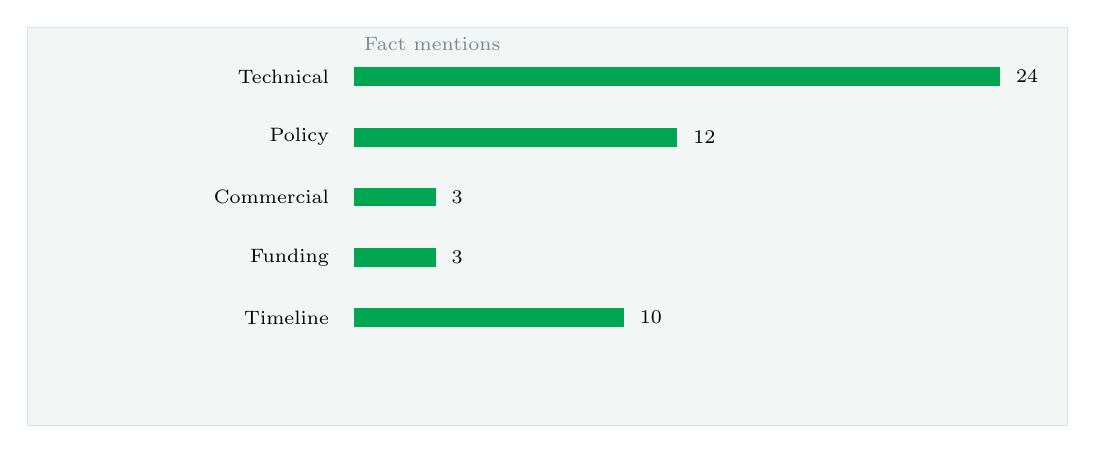
\begin{tikzpicture}[x=1cm,y=1cm]
\path[use as bounding box] (0,0) rectangle (13.20,5.05);
\fill[BOLight] (0,0) rectangle (13.20,5.05);
\draw[BOLine,line width=.35pt] (0,0) rectangle (13.20,5.05);
\node[anchor=west] at (4.15,4.85) {\scriptsize\color{BOMuted} Fact mentions};
\node[anchor=east,align=right,text width=3.93cm] at (3.95,4.43) {\scriptsize Technical};
\fill[BOLight] (4.15,4.31) rectangle (12.35,4.55);
\fill[BOGreen] (4.15,4.31) rectangle (12.35,4.55);
\node[anchor=west] at (12.43,4.43) {\scriptsize 24};
\node[anchor=east,align=right,text width=3.93cm] at (3.95,3.66) {\scriptsize Policy};
\fill[BOLight] (4.15,3.54) rectangle (12.35,3.78);
\fill[BOGreen] (4.15,3.54) rectangle (8.25,3.78);
\node[anchor=west] at (8.33,3.66) {\scriptsize 12};
\node[anchor=east,align=right,text width=3.93cm] at (3.95,2.90) {\scriptsize Commercial};
\fill[BOLight] (4.15,2.78) rectangle (12.35,3.02);
\fill[BOGreen] (4.15,2.78) rectangle (5.18,3.02);
\node[anchor=west] at (5.26,2.90) {\scriptsize 3};
\node[anchor=east,align=right,text width=3.93cm] at (3.95,2.13) {\scriptsize Funding};
\fill[BOLight] (4.15,2.01) rectangle (12.35,2.25);
\fill[BOGreen] (4.15,2.01) rectangle (5.18,2.25);
\node[anchor=west] at (5.26,2.13) {\scriptsize 3};
\node[anchor=east,align=right,text width=3.93cm] at (3.95,1.37) {\scriptsize Timeline};
\fill[BOLight] (4.15,1.25) rectangle (12.35,1.49);
\fill[BOGreen] (4.15,1.25) rectangle (7.57,1.49);
\node[anchor=west] at (7.65,1.37) {\scriptsize 10};
\end{tikzpicture}\par\vspace{2pt}
\vspace{1pt}\noindent\begin{minipage}[t]{0.56\linewidth}
{\footnotesize\color{BOText} The mix indicates whether the public record is led by technical milestones, policy institutions or commercial proof.}\par
\end{minipage}\hfill\begin{minipage}[t]{0.36\linewidth}
{\scriptsize\color{BOText}\begin{tabular}{p{31mm}>{\raggedleft\arraybackslash}p{18mm}}
\multicolumn{2}{l}{\textcolor{BOGreen}{\bfseries Visible readout}}\\[2pt]
Technical & \textbf{24}\\[1pt]
Policy & \textbf{12}\\[1pt]
Commercial & \textbf{3}\\[1pt]
Funding & \textbf{3}\\[1pt]
Timeline & \textbf{10}\\[1pt]
\end{tabular}}\par
\end{minipage}\par\vspace{1pt}
\vspace{4pt}{\footnotesize\color{BOText} The mix indicates whether the public record is led by technical milestones, policy institutions or commercial proof.}\par
{\scriptsize\color{BOMuted} Sources: science.osti.gov; energy.gov; iaea.org; iter.org.}\par

\clearpage
\label{chap:1}
\noindent\begin{tikzpicture}
\path[use as bounding box] (0,0) rectangle (\linewidth,54mm);
\clip (0,0) rectangle (\linewidth,54mm);
\node[anchor=north west,inner sep=0] at (0,54mm) {
\includegraphics[width=\linewidth]{assets/image-1.png}};
\end{tikzpicture}
\vspace{0pt}
\noindent
\begin{tikzpicture}
\fill[BOGreen] (0,0) rectangle (96mm,1.2pt);
\end{tikzpicture}\par\vspace{8pt}
{\Large\sffamily\bfseries\color{BONavy} Fusion Commercialization Is Likely Decades Away but Strategic Preparation Is Needed Now}\par\vspace{4pt}
{\sffamily\fontsize{15}{20}\selectfont\color{BOGreen} The 2022 fusion ignition breakthrough at LLNL proves scientific feasibility, but commercial power plants remain at least 15-30 years away, requiring immediate strategic positioning.}\par\vspace{9pt}
\begin{multicols}{2}
{\small The pursuit of nuclear fusion energy has entered a new era. In December 2022, Lawrence Livermore National Laboratory achieved fusion ignition, producing 2. 15 MJ of fusion energy output-a scientific first. This milestone, decades in the making, has galvanized public and private investment. Department of Energy has launched milestone-based programs to accelerate development, and private companies have raised over \$5 billion since 2020. Yet, the path to commercial power plants remains long and uncertain. ITER, the international tokamak experiment, is still under construction and not expected to produce net electricity until at least 2035.}\par
{\small For senior executives, the key insight is that fusion is not a near-term solution but a long-term strategic option. The decisions made today-whether to invest, partner, or simply monitor-will shape competitive positioning in a future energy landscape that could be transformed by fusion. This report provides a structured assessment of the technology, economics, regulation, and strategic implications, enabling informed decision-making.}\par
{\small The DOE Fusion Energy Sciences program supports a broad portfolio of research, including theory, simulation, and materials science. Private companies are pursuing diverse approaches: tokamaks (Commonwealth Fusion Systems), stellarators (Type One Energy), field-reversed configurations (TAE Technologies), and inertial confinement (Helion Energy). However, significant challenges persist. Sustaining a net-energy-producing plasma for extended periods remains unproven. Materials that can withstand the intense neutron flux in a fusion reactor are still under development. Tritium breeding-producing the fuel within the reactor-has not been demonstrated at scale.}\par
{\small ITER, the largest fusion experiment, has faced cost overruns and schedule delays. The project, originally estimated at €5 billion, now exceeds €20 billion, with first plasma expected in 2025 and full deuterium-tritium operations in 2035. These hurdles mean that even the most optimistic timelines for commercial fusion are measured in decades, not years.}\par
{\small The economic implications are clear: fusion will require sustained capital investment over multiple decades. Companies must plan for long holding periods and potential technology pivots. The strategic imperative is to build optionality through diversified bets and partnerships, rather than committing to a single approach.}\par
{\small In summary, fusion commercialization is a marathon, not a sprint. CEOs should treat fusion as a strategic hedge, not a near-term profit center. The next 2-5 years are critical for building intelligence and relationships that will enable informed decisions as the technology matures.}\par
\end{multicols}
\label{chap:1:end}

\clearpage
{\textcolor{BOGreen}{\scriptsize\bfseries EXHIBIT 5}}\par\vspace{4pt}
{\sffamily\fontsize{17}{21}\selectfont\color{BONavy} Dated facts anchor the chronology where public text permits it}\par
{\small\color{BOText} Year mentions found in public facts and source references.}\par\vspace{6pt}
\noindent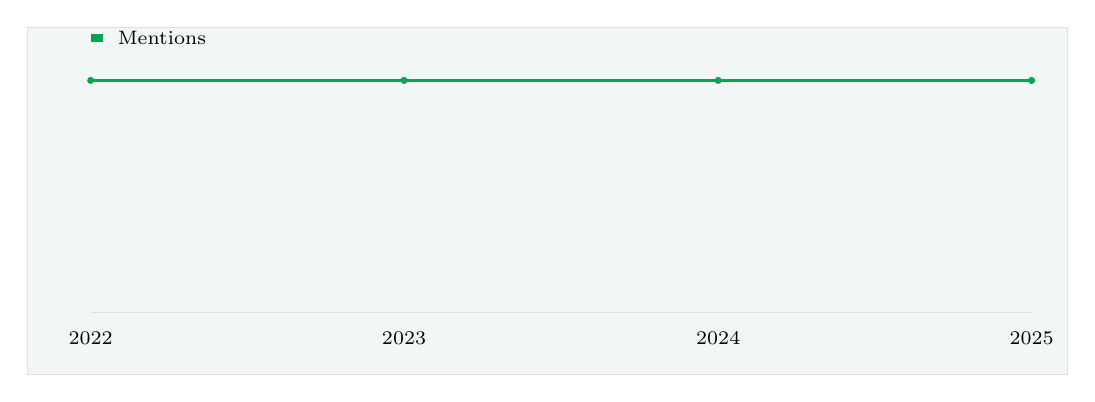
\begin{tikzpicture}[x=1cm,y=1cm]
\path[use as bounding box] (0,0) rectangle (13.20,4.40);
\fill[BOLight] (0,0) rectangle (13.20,4.40);
\draw[BOLine,line width=.35pt] (0,0) rectangle (13.20,4.40);
\draw[BOLine] (0.80,0.78) -- (12.75,0.78);
\draw[BOGreen,line width=1.1pt] (0.80,3.73) -- (4.78,3.73) -- (8.77,3.73) -- (12.75,3.73);
\fill[BOGreen] (0.80,3.73) circle (.045);
\fill[BOGreen] (4.78,3.73) circle (.045);
\fill[BOGreen] (8.77,3.73) circle (.045);
\fill[BOGreen] (12.75,3.73) circle (.045);
\node[anchor=north,align=center,text width=1.8cm] at (0.80,0.66) {\scriptsize 2022};
\node[anchor=north,align=center,text width=1.8cm] at (4.78,0.66) {\scriptsize 2023};
\node[anchor=north,align=center,text width=1.8cm] at (8.77,0.66) {\scriptsize 2024};
\node[anchor=north,align=center,text width=1.8cm] at (12.75,0.66) {\scriptsize 2025};
\fill[BOGreen] (0.80,4.22) rectangle (0.96,4.32);
\node[anchor=west] at (1.02,4.27) {\scriptsize Mentions};
\end{tikzpicture}\par\vspace{2pt}
\vspace{1pt}\noindent\begin{minipage}[t]{0.56\linewidth}
{\footnotesize\color{BOText} Timeline claims are stronger when they can be tied to explicit years rather than broad commercialization language.}\par
\end{minipage}\hfill\begin{minipage}[t]{0.36\linewidth}
{\scriptsize\color{BOText}\begin{tabular}{p{31mm}>{\raggedleft\arraybackslash}p{18mm}}
\multicolumn{2}{l}{\textcolor{BOGreen}{\bfseries Visible readout}}\\[2pt]
2022 & \textbf{1}\\[1pt]
2023 & \textbf{1}\\[1pt]
2024 & \textbf{1}\\[1pt]
2025 & \textbf{1}\\[1pt]
\end{tabular}}\par
\end{minipage}\par\vspace{1pt}
\vspace{4pt}{\footnotesize\color{BOText} Timeline claims are stronger when they can be tied to explicit years rather than broad commercialization language.}\par
{\scriptsize\color{BOMuted} Sources: science.osti.gov; energy.gov; iaea.org; iter.org.}\par
\vspace{9pt}\textcolor{BOLine}{\rule{\linewidth}{0.3pt}}\vspace{8pt}
{\textcolor{BOGreen}{\scriptsize\bfseries EXHIBIT 6}}\par\vspace{4pt}
{\sffamily\fontsize{17}{21}\selectfont\color{BONavy} Source type mix separates full pages from thin snippets}\par
{\small\color{BOText} Public sources by content form and authority flag.}\par\vspace{6pt}
\noindent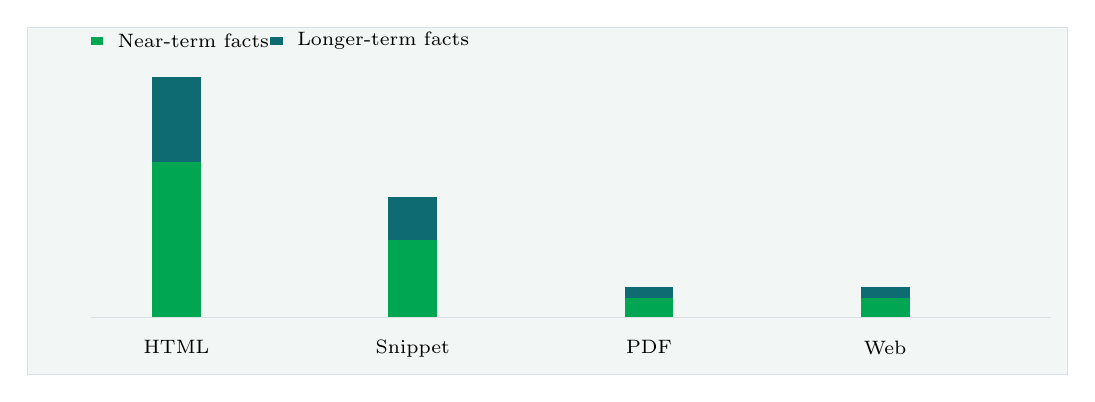
\begin{tikzpicture}[x=1cm,y=1cm]
\path[use as bounding box] (0,0) rectangle (13.20,4.40);
\fill[BOLight] (0,0) rectangle (13.20,4.40);
\draw[BOLine,line width=.35pt] (0,0) rectangle (13.20,4.40);
\draw[BOLine] (0.80,0.72) -- (13.00,0.72);
\fill[BOGreen] (1.58,0.72) rectangle (2.20,2.69);
\fill[BOBlue] (1.58,2.69) rectangle (2.20,3.77);
\node[anchor=north,align=center,text width=2.76cm] at (1.89,0.55) {\scriptsize HTML};
\fill[BOGreen] (4.58,0.72) rectangle (5.20,1.70);
\fill[BOBlue] (4.58,1.70) rectangle (5.20,2.25);
\node[anchor=north,align=center,text width=2.76cm] at (4.89,0.55) {\scriptsize Snippet};
\fill[BOGreen] (7.58,0.72) rectangle (8.20,0.97);
\fill[BOBlue] (7.58,0.97) rectangle (8.20,1.11);
\node[anchor=north,align=center,text width=2.76cm] at (7.89,0.55) {\scriptsize PDF};
\fill[BOGreen] (10.58,0.72) rectangle (11.20,0.97);
\fill[BOBlue] (10.58,0.97) rectangle (11.20,1.11);
\node[anchor=north,align=center,text width=2.76cm] at (10.89,0.55) {\scriptsize Web};
\fill[BOGreen] (0.80,4.18) rectangle (0.96,4.28);
\node[anchor=west] at (1.02,4.23) {\scriptsize Near-term facts};
\fill[BOBlue] (3.08,4.18) rectangle (3.24,4.28);
\node[anchor=west] at (3.30,4.23) {\scriptsize Longer-term facts};
\end{tikzpicture}\par\vspace{2pt}
\vspace{1pt}\noindent\begin{minipage}[t]{0.56\linewidth}
{\footnotesize\color{BOText} Pages and PDFs with extractable body text can support richer prose than snippets that carry only limited context.}\par
\end{minipage}\hfill\begin{minipage}[t]{0.36\linewidth}
{\scriptsize\color{BOText}\begin{tabular}{p{31mm}>{\raggedleft\arraybackslash}p{18mm}}
\multicolumn{2}{l}{\textcolor{BOGreen}{\bfseries Visible readout}}\\[2pt]
HTML & \textbf{37.2}\\[1pt]
Snippet & \textbf{18.6}\\[1pt]
PDF & \textbf{4.7}\\[1pt]
Web & \textbf{4.7}\\[1pt]
\end{tabular}}\par
\end{minipage}\par\vspace{1pt}
\vspace{4pt}{\footnotesize\color{BOText} Pages and PDFs with extractable body text can support richer prose than snippets that carry only limited context.}\par
{\scriptsize\color{BOMuted} Sources: science.osti.gov; energy.gov; iaea.org; iter.org.}\par

\clearpage
\label{chap:2}
\noindent\begin{tikzpicture}
\path[use as bounding box] (0,0) rectangle (\linewidth,54mm);
\clip (0,0) rectangle (\linewidth,54mm);
\node[anchor=north west,inner sep=0] at (0,54mm) {
\includegraphics[width=\linewidth]{assets/image-2.png}};
\end{tikzpicture}
\vspace{0pt}
\noindent
\begin{tikzpicture}
\fill[BOGreen] (0,0) rectangle (96mm,1.2pt);
\end{tikzpicture}\par\vspace{8pt}
{\Large\sffamily\bfseries\color{BONavy} Technology Progress Is Accelerating but Significant Hurdles Remain}\par\vspace{4pt}
{\sffamily\fontsize{15}{20}\selectfont\color{BOGreen} While fusion experiments have achieved historic milestones, sustained net energy gain, materials durability, and tritium breeding remain unproven at commercial scale.}\par\vspace{9pt}
\begin{multicols}{2}
{\small Fusion research has made remarkable strides. The 2022 ignition experiment at LLNL demonstrated scientific breakeven, a goal pursued for 60 years. The DOE\BOApos{}s Fusion Energy Sciences program supports a broad portfolio of research, including theory, simulation, and materials science. Private companies are pursuing diverse approaches: tokamaks (Commonwealth Fusion Systems), stellarators (Type One Energy), field-reversed configurations (TAE Technologies), and inertial confinement (Helion Energy).}\par
{\small However, significant challenges persist. Sustaining a net-energy-producing plasma for extended periods remains unproven. Materials that can withstand the intense neutron flux in a fusion reactor are still under development. Tritium breeding-producing the fuel within the reactor-has not been demonstrated at scale. ITER, the largest fusion experiment, has faced cost overruns and schedule delays. The project, originally estimated at €5 billion, now exceeds €20 billion, with first plasma expected in 2025 and full deuterium-tritium operations in 2035.}\par
{\small These hurdles mean that even the most optimistic timelines for commercial fusion are measured in decades, not years. For investors, this implies that fusion is a long-duration asset class with high technology risk. Diversification across multiple approaches (magnetic confinement, inertial confinement, alternative concepts) can mitigate some risk, but the sector remains binary in nature.}\par
{\small The DOE Milestone-Based Fusion Development Program is designed to de-risk technology by providing public funding for key milestones. This program, along with ARPA-E initiatives, helps share the financial burden with private companies. Companies should monitor these programs for partnership opportunities.}\par
{\small From a commercial perspective, the key question is not whether fusion will work, but when and at what cost. The answer will determine whether fusion becomes a mainstream energy source or a niche technology. Early movers who invest in R\&D partnerships and talent acquisition will be better positioned to capitalize on breakthroughs.}\par
{\small In conclusion, technology progress is real but incremental. CEOs should set realistic expectations with boards and investors, emphasizing that fusion is a long-term play requiring patience and sustained commitment.}\par
\end{multicols}
\label{chap:2:end}

\clearpage
{\textcolor{BOGreen}{\scriptsize\bfseries EXHIBIT 7}}\par\vspace{4pt}
{\sffamily\fontsize{17}{21}\selectfont\color{BONavy} Business relevance depends on numbers, dates and commercial proof}\par
{\small\color{BOText} Numeric, dated and commercial references across the main narrative.}\par\vspace{6pt}
\noindent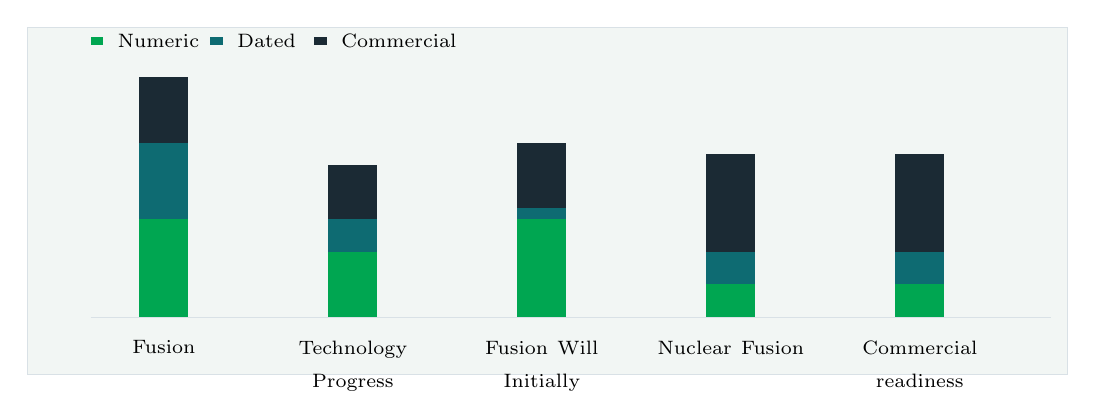
\begin{tikzpicture}[x=1cm,y=1cm]
\path[use as bounding box] (0,0) rectangle (13.20,4.40);
\fill[BOLight] (0,0) rectangle (13.20,4.40);
\draw[BOLine,line width=.35pt] (0,0) rectangle (13.20,4.40);
\draw[BOLine] (0.80,0.72) -- (13.00,0.72);
\fill[BOGreen] (1.42,0.72) rectangle (2.04,1.97);
\fill[BOBlue] (1.42,1.97) rectangle (2.04,2.94);
\fill[BONavy] (1.42,2.94) rectangle (2.04,3.77);
\node[anchor=north,align=center,text width=2.21cm] at (1.73,0.55) {\scriptsize Fusion};
\fill[BOGreen] (3.82,0.72) rectangle (4.44,1.55);
\fill[BOBlue] (3.82,1.55) rectangle (4.44,1.97);
\fill[BONavy] (3.82,1.97) rectangle (4.44,2.66);
\node[anchor=north,align=center,text width=2.21cm] at (4.13,0.55) {\scriptsize Technology Progress};
\fill[BOGreen] (6.22,0.72) rectangle (6.84,1.97);
\fill[BOBlue] (6.22,1.97) rectangle (6.84,2.11);
\fill[BONavy] (6.22,2.11) rectangle (6.84,2.94);
\node[anchor=north,align=center,text width=2.21cm] at (6.53,0.55) {\scriptsize Fusion Will Initially};
\fill[BOGreen] (8.62,0.72) rectangle (9.24,1.14);
\fill[BOBlue] (8.62,1.14) rectangle (9.24,1.55);
\fill[BONavy] (8.62,1.55) rectangle (9.24,2.80);
\node[anchor=north,align=center,text width=2.21cm] at (8.93,0.55) {\scriptsize Nuclear Fusion};
\fill[BOGreen] (11.02,0.72) rectangle (11.64,1.14);
\fill[BOBlue] (11.02,1.14) rectangle (11.64,1.55);
\fill[BONavy] (11.02,1.55) rectangle (11.64,2.80);
\node[anchor=north,align=center,text width=2.21cm] at (11.33,0.55) {\scriptsize Commercial readiness};
\fill[BOGreen] (0.80,4.18) rectangle (0.96,4.28);
\node[anchor=west] at (1.02,4.23) {\scriptsize Numeric};
\fill[BOBlue] (2.32,4.18) rectangle (2.48,4.28);
\node[anchor=west] at (2.54,4.23) {\scriptsize Dated};
\fill[BONavy] (3.64,4.18) rectangle (3.80,4.28);
\node[anchor=west] at (3.86,4.23) {\scriptsize Commercial};
\end{tikzpicture}\par\vspace{2pt}
\vspace{1pt}\noindent\begin{minipage}[t]{0.56\linewidth}
{\footnotesize\color{BOText} A board reader needs later pages to carry the same factual weight as the opening argument, especially around numbers and dated milestones.}\par
\end{minipage}\hfill\begin{minipage}[t]{0.36\linewidth}
{\scriptsize\color{BOText}\begin{tabular}{p{31mm}>{\raggedleft\arraybackslash}p{18mm}}
\multicolumn{2}{l}{\textcolor{BOGreen}{\bfseries Visible readout}}\\[2pt]
Fusion & \textbf{22}\\[1pt]
Technology Progress Is & \textbf{14}\\[1pt]
Fusion Will Initially & \textbf{16}\\[1pt]
Nuclear Fusion & \textbf{15}\\[1pt]
Commercial readiness & \textbf{15}\\[1pt]
\end{tabular}}\par
\end{minipage}\par\vspace{1pt}
\vspace{4pt}{\footnotesize\color{BOText} A board reader needs later pages to carry the same factual weight as the opening argument, especially around numbers and dated milestones.}\par
{\scriptsize\color{BOMuted} Sources: public references and report analysis.}\par
\vspace{9pt}\textcolor{BOLine}{\rule{\linewidth}{0.3pt}}\vspace{8pt}
{\textcolor{BOGreen}{\scriptsize\bfseries EXHIBIT 8}}\par\vspace{4pt}
{\sffamily\fontsize{17}{21}\selectfont\color{BONavy} Evidence support differs by business question}\par
{\small\color{BOText} A compact support matrix for the main executive questions.}\par\vspace{6pt}
\noindent\fcolorbox{BOLine}{BOLight}{\begin{minipage}{0.96\linewidth}\vspace{4pt}{\scriptsize\begin{tabular}{p{38mm}>{\centering\arraybackslash}p{21mm}>{\centering\arraybackslash}p{21mm}>{\centering\arraybackslash}p{21mm}>{\centering\arraybackslash}p{21mm}}
 & {\bfseries Sources} & {\bfseries Numbers} & {\bfseries Dates} & {\bfseries Business tie} \\
\hline
{\bfseries Fusion Commercialization Is.} & \colorbox{BOGreen}{\textcolor{white}{\strut\hspace{5pt}4\hspace{5pt}}} & \colorbox{BOGreen}{\textcolor{white}{\strut\hspace{5pt}5\hspace{5pt}}} & \colorbox{BOGreen}{\textcolor{white}{\strut\hspace{5pt}5\hspace{5pt}}} & \colorbox{BOGreen}{\textcolor{white}{\strut\hspace{5pt}5\hspace{5pt}}} \\
{\bfseries Technology Progress Is Acce.} & \colorbox{BOGreen}{\textcolor{white}{\strut\hspace{5pt}4\hspace{5pt}}} & \colorbox{BOGreen}{\textcolor{white}{\strut\hspace{5pt}5\hspace{5pt}}} & \colorbox{BOBlue}{\textcolor{white}{\strut\hspace{5pt}3\hspace{5pt}}} & \colorbox{BOGreen}{\textcolor{white}{\strut\hspace{5pt}5\hspace{5pt}}} \\
{\bfseries Fusion Will Initially Be Ex.} & \colorbox{BOGreen}{\textcolor{white}{\strut\hspace{5pt}4\hspace{5pt}}} & \colorbox{BOGreen}{\textcolor{white}{\strut\hspace{5pt}5\hspace{5pt}}} & \colorbox{BOLight}{\textcolor{BOText}{\strut\hspace{5pt}1\hspace{5pt}}} & \colorbox{BOGreen}{\textcolor{white}{\strut\hspace{5pt}5\hspace{5pt}}} \\
{\bfseries Nuclear Fusion Commercializ.} & \colorbox{BOGreen}{\textcolor{white}{\strut\hspace{5pt}4\hspace{5pt}}} & \colorbox{BOBlue}{\textcolor{white}{\strut\hspace{5pt}3\hspace{5pt}}} & \colorbox{BOBlue}{\textcolor{white}{\strut\hspace{5pt}3\hspace{5pt}}} & \colorbox{BOGreen}{\textcolor{white}{\strut\hspace{5pt}5\hspace{5pt}}} \\
{\bfseries Commercial readiness depend.} & \colorbox{BOGreen}{\textcolor{white}{\strut\hspace{5pt}4\hspace{5pt}}} & \colorbox{BOBlue}{\textcolor{white}{\strut\hspace{5pt}3\hspace{5pt}}} & \colorbox{BOBlue}{\textcolor{white}{\strut\hspace{5pt}3\hspace{5pt}}} & \colorbox{BOGreen}{\textcolor{white}{\strut\hspace{5pt}5\hspace{5pt}}} \\
\end{tabular}}\vspace{4pt}\end{minipage}}\par\vspace{2pt}
\vspace{1pt}\noindent\begin{minipage}[t]{0.56\linewidth}
{\footnotesize\color{BOText} The strongest pages connect source depth with numbers, dates and direct business implications.}\par
\end{minipage}\hfill\begin{minipage}[t]{0.36\linewidth}
{\scriptsize\color{BOText}\begin{tabular}{p{31mm}>{\raggedleft\arraybackslash}p{18mm}}
\multicolumn{2}{l}{\textcolor{BOGreen}{\bfseries Matrix readout}}\\[2pt]
Fusion & \textbf{4 / 5}\\[1pt]
Technology Progress & \textbf{4 / 5}\\[1pt]
Fusion Will Initially & \textbf{4 / 5}\\[1pt]
Nuclear Fusion & \textbf{4 / 3}\\[1pt]
\end{tabular}}\par
\end{minipage}\par\vspace{1pt}
\vspace{4pt}{\footnotesize\color{BOText} The strongest pages connect source depth with numbers, dates and direct business implications.}\par
{\scriptsize\color{BOMuted} Sources: science.osti.gov; energy.gov; iaea.org; iter.org.}\par

\clearpage
\label{chap:3}
\noindent\begin{tikzpicture}
\path[use as bounding box] (0,0) rectangle (\linewidth,54mm);
\clip (0,0) rectangle (\linewidth,54mm);
\node[anchor=north west,inner sep=0] at (0,54mm) {
\includegraphics[width=\linewidth]{assets/image-3.png}};
\end{tikzpicture}
\vspace{0pt}
\noindent
\begin{tikzpicture}
\fill[BOGreen] (0,0) rectangle (96mm,1.2pt);
\end{tikzpicture}\par\vspace{8pt}
{\Large\sffamily\bfseries\color{BONavy} Fusion Will Initially Be Expensive but Could Become Competitive with Baseload Power}\par\vspace{4pt}
{\sffamily\fontsize{15}{20}\selectfont\color{BOGreen} First-of-a-kind fusion plants will have high LCOE (\$100-200/MWh), but costs could fall to \$50-100/MWh by 2050, making fusion competitive with nuclear and gas with carbon capture.}\par\vspace{9pt}
\begin{multicols}{2}
{\small The economics of fusion are highly uncertain. Early estimates from the National Academies and industry analysts suggest that the levelized cost of energy (LCOE) for first-of-a-kind fusion plants could range from \$100-200/MWh, significantly higher than current solar (\$30-50/MWh) and wind (\$40-60/MWh). However, as the technology matures and scales, LCOE could fall to \$50-100/MWh, making it competitive with nuclear fission and natural gas with carbon capture.}\par
{\small Fusion\BOApos{}s key economic advantage is its high capacity factor (90\%+), providing reliable baseload power. This contrasts with intermittent renewables, which require storage or backup. Fusion also has low fuel costs (deuterium and lithium are abundant) and no carbon emissions. However, capital costs are expected to be very high, potentially \$5-10 billion per GW, similar to fission.}\par
{\small For investors, the economic case for fusion hinges on cost reduction through learning and scale. The first few plants will likely require government subsidies or power purchase agreements at premium prices. As the industry matures, costs could decline, but the pace is uncertain. Companies should model a range of scenarios, from optimistic (rapid cost decline) to pessimistic (fusion remains niche).}\par
{\small Fusion\BOApos{}s competitiveness also depends on the evolution of alternative technologies. If renewables plus storage become cheaper and more reliable, fusion\BOApos{}s market may be limited to specific applications like industrial heat or hydrogen production. Conversely, if carbon pricing or grid reliability concerns increase, fusion could become more attractive.}\par
{\small For partner strategy, in summary, fusion economics are a long-term bet. Companies should not expect fusion to compete with solar and wind in the near term, but it could play a role in a diversified net-zero portfolio by mid-century. Strategic investments should be sized accordingly.}\par
{\small Every opportunity eventually returns to cost, revenue, margin, cash flow and timing. If sourced evidence does not support market size, ROI, unit economics or share, those items should remain explicit assumptions rather than conclusions.}\par
\end{multicols}
\label{chap:3:end}

\clearpage
\label{chap:4}
\noindent\begin{tikzpicture}
\path[use as bounding box] (0,0) rectangle (\linewidth,54mm);
\clip (0,0) rectangle (\linewidth,54mm);
\node[anchor=north west,inner sep=0] at (0,54mm) {
\includegraphics[width=\linewidth]{assets/image-4.png}};
\end{tikzpicture}
\vspace{0pt}
\noindent
\begin{tikzpicture}
\fill[BOGreen] (0,0) rectangle (96mm,1.2pt);
\end{tikzpicture}\par\vspace{8pt}
{\Large\sffamily\bfseries\color{BONavy} Nuclear Fusion Commercialization Outlook and Strategic Implications should be managed as a staged strategic option, not a binary bet}\par\vspace{4pt}
{\sffamily\fontsize{15}{20}\selectfont\color{BOGreen} The CEO question is which moves are safe now and which should wait for stronger proof.}\par\vspace{9pt}
\begin{multicols}{2}
{\small Nuclear Fusion Commercialization Outlook and Strategic Implications is easier to misread when it is framed as a yes-or-no bet. The better reading separates near-term learning moves, option-building partnerships and commitments that would require stronger commercial proof.}\par
{\small For the board, the immediate management question is not whether the opportunity is exciting; it is whether budget, partner access or management attention should be committed now. Low-cost validation can start early, while larger capital commitments should wait for customer, cost, financing, regulatory or operating proof.}\par
{\small For customer strategy, the current source base is useful but incomplete. A public source anchors this point: The Department of Energy has been a leader in fusion energy research since the 1950s and supports groundbreaking advances today. A quarterly review rhythm is more useful than a one-time verdict because the facts that matter will change as customers, regulators and suppliers move.}\par
{\small The executive question around Nuclear Fusion Commercialization Outlook and Strategic Implications should be managed as a staged strategic option, not. is practical: which commitments create learning without locking the company into a cost curve, customer promise or regulatory position that the facts cannot yet support.}\par
{\small Capital tied to Nuclear Fusion Commercialization Outlook and Strategic Implications should be managed as a staged strategic option, not. should move only when proof improves along the dimensions that change a business case: customer demand, cost position, financing availability, regulatory path and delivery capability. If those facts do not improve, larger exposure creates lock-in rather than conviction.}\par
{\small The strongest public fact pattern for Nuclear Fusion Commercialization Outlook and Strategic Implications should be managed as a staged strategic option, not. is narrow but useful: The Department of Energy has been a leader in fusion energy research since the 1950s and supports groundbreaking advances today. It should shape the next customer, cost or partner question without being stretched into proof of commercial scale.}\par
\end{multicols}
\label{chap:4:end}

\clearpage
{\textcolor{BOGreen}{\scriptsize\bfseries EXHIBIT 9}}\par\vspace{4pt}
{\sffamily\fontsize{17}{21}\selectfont\color{BONavy} Domain map separates institutional authority from factual detail}\par
{\small\color{BOText} Each point is a public domain positioned by authority and available factual detail.}\par\vspace{6pt}
\noindent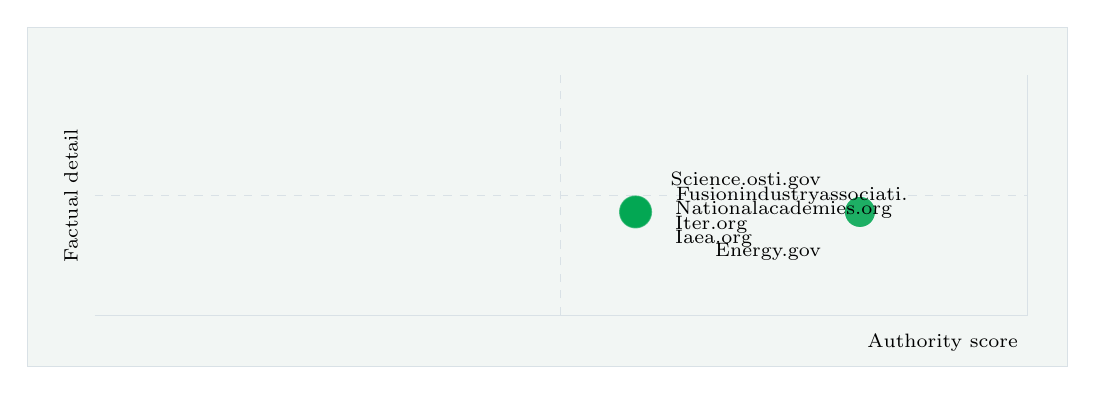
\begin{tikzpicture}[x=1cm,y=1cm]
\path[use as bounding box] (0,0) rectangle (13.20,4.30);
\fill[BOLight] (0,0) rectangle (13.20,4.30);
\draw[BOLine,line width=.35pt] (0,0) rectangle (13.20,4.30);
\draw[BOLine] (0.85,0.65) -- (12.70,0.65) -- (12.70,3.70);
\draw[BOLine,dashed] (0.85,2.17) -- (12.70,2.17);
\draw[BOLine,dashed] (6.77,0.65) -- (6.77,3.70);
\fill[BOGreen,opacity=.65] (10.57,1.96) circle (0.19);
\node[anchor=east,align=right,text width=2.10cm] at (10.20,2.35) {\scriptsize Science.osti.gov};
\fill[BOGreen,opacity=.65] (10.57,1.96) circle (0.19);
\node[anchor=east,align=right,text width=2.10cm] at (10.20,1.46) {\scriptsize Energy.gov};
\fill[BOGreen,opacity=.65] (7.72,1.96) circle (0.19);
\node[anchor=west,align=left,text width=2.10cm] at (8.10,1.62) {\scriptsize Iaea.org};
\fill[BOGreen,opacity=.65] (7.72,1.96) circle (0.20);
\node[anchor=west,align=left,text width=2.10cm] at (8.10,1.80) {\scriptsize Iter.org};
\fill[BOGreen,opacity=.65] (7.72,1.96) circle (0.20);
\node[anchor=west,align=left,text width=2.10cm] at (8.10,1.99) {\scriptsize Nationalacademies.org};
\fill[BOGreen,opacity=.65] (7.72,1.96) circle (0.21);
\node[anchor=west,align=left,text width=2.10cm] at (8.11,2.17) {\scriptsize Fusionindustryassociati.};
\node[anchor=north east] at (12.70,0.53) {\scriptsize Authority score};
\node[anchor=center,rotate=90] at (0.55,2.17) {\scriptsize Factual detail};
\end{tikzpicture}\par\vspace{2pt}
\vspace{1pt}\noindent\begin{minipage}[t]{0.56\linewidth}
{\footnotesize\color{BOText} Upper-right domains deserve more weight in the narrative because they combine credibility with extractable factual detail.}\par
\end{minipage}\hfill\begin{minipage}[t]{0.36\linewidth}
{\scriptsize\color{BOText}\begin{tabular}{p{31mm}>{\raggedleft\arraybackslash}p{18mm}}
\multicolumn{2}{l}{\textcolor{BOGreen}{\bfseries Position}}\\[2pt]
Science.osti.gov & \textbf{82 / 43}\\[1pt]
Energy.gov & \textbf{82 / 43}\\[1pt]
Iaea.org & \textbf{58 / 43}\\[1pt]
Iter.org & \textbf{58 / 43}\\[1pt]
Nationalacademies.org & \textbf{58 / 43}\\[1pt]
\end{tabular}}\par
\end{minipage}\par\vspace{1pt}
\vspace{4pt}{\footnotesize\color{BOText} Upper-right domains deserve more weight in the narrative because they combine credibility with extractable factual detail.}\par
{\scriptsize\color{BOMuted} Sources: science.osti.gov; energy.gov; iaea.org; iter.org.}\par
\vspace{9pt}\textcolor{BOLine}{\rule{\linewidth}{0.3pt}}\vspace{8pt}
{\textcolor{BOGreen}{\scriptsize\bfseries EXHIBIT 10}}\par\vspace{4pt}
{\sffamily\fontsize{17}{21}\selectfont\color{BONavy} Commercial quantification remains thinner than milestone evidence}\par
{\small\color{BOText} Numeric facts are grouped by the type of decision they can support.}\par\vspace{6pt}
\noindent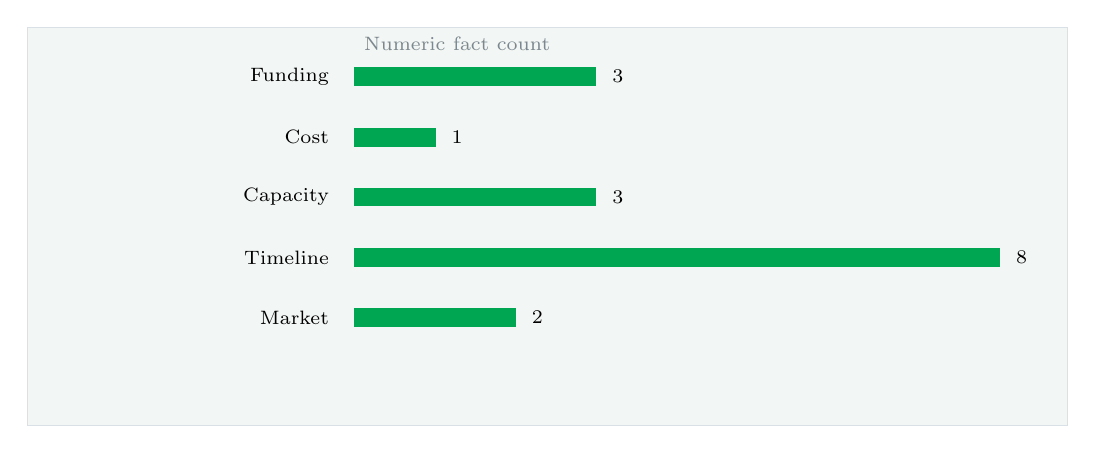
\begin{tikzpicture}[x=1cm,y=1cm]
\path[use as bounding box] (0,0) rectangle (13.20,5.05);
\fill[BOLight] (0,0) rectangle (13.20,5.05);
\draw[BOLine,line width=.35pt] (0,0) rectangle (13.20,5.05);
\node[anchor=west] at (4.15,4.85) {\scriptsize\color{BOMuted} Numeric fact count};
\node[anchor=east,align=right,text width=3.93cm] at (3.95,4.43) {\scriptsize Funding};
\fill[BOLight] (4.15,4.31) rectangle (12.35,4.55);
\fill[BOGreen] (4.15,4.31) rectangle (7.22,4.55);
\node[anchor=west] at (7.30,4.43) {\scriptsize 3};
\node[anchor=east,align=right,text width=3.93cm] at (3.95,3.66) {\scriptsize Cost};
\fill[BOLight] (4.15,3.54) rectangle (12.35,3.78);
\fill[BOGreen] (4.15,3.54) rectangle (5.18,3.78);
\node[anchor=west] at (5.26,3.66) {\scriptsize 1};
\node[anchor=east,align=right,text width=3.93cm] at (3.95,2.90) {\scriptsize Capacity};
\fill[BOLight] (4.15,2.78) rectangle (12.35,3.02);
\fill[BOGreen] (4.15,2.78) rectangle (7.22,3.02);
\node[anchor=west] at (7.30,2.90) {\scriptsize 3};
\node[anchor=east,align=right,text width=3.93cm] at (3.95,2.13) {\scriptsize Timeline};
\fill[BOLight] (4.15,2.01) rectangle (12.35,2.25);
\fill[BOGreen] (4.15,2.01) rectangle (12.35,2.25);
\node[anchor=west] at (12.43,2.13) {\scriptsize 8};
\node[anchor=east,align=right,text width=3.93cm] at (3.95,1.37) {\scriptsize Market};
\fill[BOLight] (4.15,1.25) rectangle (12.35,1.49);
\fill[BOGreen] (4.15,1.25) rectangle (6.20,1.49);
\node[anchor=west] at (6.28,1.37) {\scriptsize 2};
\end{tikzpicture}\par\vspace{2pt}
\vspace{1pt}\noindent\begin{minipage}[t]{0.56\linewidth}
{\footnotesize\color{BOText} A CEO can act faster when funding, cost, capacity and market claims are quantified instead of only described qualitatively.}\par
\end{minipage}\hfill\begin{minipage}[t]{0.36\linewidth}
{\scriptsize\color{BOText}\begin{tabular}{p{31mm}>{\raggedleft\arraybackslash}p{18mm}}
\multicolumn{2}{l}{\textcolor{BOGreen}{\bfseries Visible readout}}\\[2pt]
Funding & \textbf{3}\\[1pt]
Cost & \textbf{1}\\[1pt]
Capacity & \textbf{3}\\[1pt]
Timeline & \textbf{8}\\[1pt]
Market & \textbf{2}\\[1pt]
\end{tabular}}\par
\end{minipage}\par\vspace{1pt}
\vspace{4pt}{\footnotesize\color{BOText} A CEO can act faster when funding, cost, capacity and market claims are quantified instead of only described qualitatively.}\par
{\scriptsize\color{BOMuted} Sources: science.osti.gov; energy.gov; iaea.org; iter.org.}\par

\clearpage
\label{chap:5}
\noindent\begin{tikzpicture}
\path[use as bounding box] (0,0) rectangle (\linewidth,54mm);
\clip (0,0) rectangle (\linewidth,54mm);
\node[anchor=north west,inner sep=0] at (0,54mm) {
\includegraphics[width=\linewidth]{assets/image-5.png}};
\end{tikzpicture}
\vspace{0pt}
\noindent
\begin{tikzpicture}
\fill[BOGreen] (0,0) rectangle (96mm,1.2pt);
\end{tikzpicture}\par\vspace{8pt}
{\Large\sffamily\bfseries\color{BONavy} Commercial readiness depends on bankability, deliverability and repeat customer proof}\par\vspace{4pt}
{\sffamily\fontsize{15}{20}\selectfont\color{BOGreen} Technical feasibility matters only when it changes customer value, cost position and execution confidence.}\par\vspace{9pt}
\begin{multicols}{2}
{\small For the board, commercial readiness should be judged through customer adoption, cost structure, delivery cycle, service capability and financing availability. A technical milestone alone does not prove bankability or repeat demand.}\par
{\small From an investor lens, every major assumption needs a verifiable claim behind it: target customer, buying trigger, budget owner, substitute, use case and payback path. Where sourced evidence is missing, the claim should remain directional.}\par
{\small A more robust path is to build credible proof through pilots, partner diligence and third-party validation before moving into larger commitments.}\par
{\small At the portfolio level, the executive question around Commercial readiness depends on bankability, deliverability and repeat customer proof is practical: which commitments create learning without locking the company into a cost curve, customer promise or regulatory position that the facts cannot yet support.}\par
{\small Capital tied to Commercial readiness depends on bankability, deliverability and repeat customer proof should move only when proof improves along the dimensions that change a business case: customer demand, cost position, financing availability, regulatory path and delivery capability. If those facts do not improve, larger exposure creates lock-in rather than conviction.}\par
{\small For operating teams, the strongest public fact pattern for Commercial readiness depends on bankability, deliverability and repeat customer proof is narrow but useful: The Department of Energy has been a leader in fusion energy research since the 1950s and supports groundbreaking advances today. It should shape the next customer, cost or partner question without being stretched into proof of commercial scale.}\par
\end{multicols}
\label{chap:5:end}

\clearpage
\label{chap:6}
\noindent\begin{tikzpicture}
\path[use as bounding box] (0,0) rectangle (\linewidth,54mm);
\clip (0,0) rectangle (\linewidth,54mm);
\node[anchor=north west,inner sep=0] at (0,54mm) {
\includegraphics[width=\linewidth]{assets/image-6.png}};
\end{tikzpicture}
\vspace{0pt}
\noindent
\begin{tikzpicture}
\fill[BOGreen] (0,0) rectangle (96mm,1.2pt);
\end{tikzpicture}\par\vspace{8pt}
{\Large\sffamily\bfseries\color{BONavy} Cost, return and timing will determine the real deployment window}\par\vspace{4pt}
{\sffamily\fontsize{15}{20}\selectfont\color{BOGreen} Market size should not enter an investment case until the cost and return logic can be checked.}\par\vspace{9pt}
\begin{multicols}{2}
{\small In timing terms, every opportunity eventually returns to cost, revenue, margin, cash flow and timing. If sourced evidence does not support market size, ROI, unit economics or share, those items should remain explicit assumptions rather than conclusions.}\par
{\small For risk owners, near-term action should focus on verifiable cost drivers and customer willingness to pay instead of relying on optimistic long-range scenarios. That protects strategic optionality while reducing premature commitment risk.}\par
{\small In timing terms, as cost, customer and financing evidence improves, management can shift resources from monitoring and partnerships toward pilots or scaled deployment.}\par
{\small In timing terms, the executive question around Cost, return and timing will determine the real deployment window is practical: which commitments create learning without locking the company into a cost curve, customer promise or regulatory position that the facts cannot yet support.}\par
{\small In timing terms, capital tied to Cost, return and timing will determine the real deployment window should move only when proof improves along the dimensions that change a business case: customer demand, cost position, financing availability, regulatory path and delivery capability. If those facts do not improve, larger exposure creates lock-in rather than conviction.}\par
{\small For risk owners, the strongest public fact pattern for Cost, return and timing will determine the real deployment window is narrow but useful: The Department of Energy has been a leader in fusion energy research since the 1950s and supports groundbreaking advances today. It should shape the next customer, cost or partner question without being stretched into proof of commercial scale.}\par
\end{multicols}
\label{chap:6:end}

\clearpage
{\textcolor{BOGreen}{\scriptsize\bfseries EXHIBIT 11}}\par\vspace{4pt}
{\sffamily\fontsize{17}{21}\selectfont\color{BONavy} Institution roles clarify which claims each source can support}\par
{\small\color{BOText} Rows classify public institutions; columns show their most useful contribution.}\par\vspace{6pt}
\noindent\fcolorbox{BOLine}{BOLight}{\begin{minipage}{0.96\linewidth}\vspace{4pt}{\scriptsize\begin{tabular}{p{38mm}>{\centering\arraybackslash}p{21mm}>{\centering\arraybackslash}p{21mm}>{\centering\arraybackslash}p{21mm}>{\centering\arraybackslash}p{21mm}}
 & {\bfseries Policy} & {\bfseries Technology} & {\bfseries Market} & {\bfseries Timeline} \\
\hline
{\bfseries Government} & \colorbox{BOGreen}{\textcolor{white}{\strut\hspace{5pt}5\hspace{5pt}}} & \colorbox{BOBlue}{\textcolor{white}{\strut\hspace{5pt}3\hspace{5pt}}} & \colorbox{BOLight}{\textcolor{BOText}{\strut\hspace{5pt}2\hspace{5pt}}} & \colorbox{BOGreen}{\textcolor{white}{\strut\hspace{5pt}4\hspace{5pt}}} \\
{\bfseries Research} & \colorbox{BOLight}{\textcolor{BOText}{\strut\hspace{5pt}2\hspace{5pt}}} & \colorbox{BOGreen}{\textcolor{white}{\strut\hspace{5pt}5\hspace{5pt}}} & \colorbox{BOLight}{\textcolor{BOText}{\strut\hspace{5pt}2\hspace{5pt}}} & \colorbox{BOGreen}{\textcolor{white}{\strut\hspace{5pt}4\hspace{5pt}}} \\
{\bfseries Industry} & \colorbox{BOLight}{\textcolor{BOText}{\strut\hspace{5pt}2\hspace{5pt}}} & \colorbox{BOBlue}{\textcolor{white}{\strut\hspace{5pt}3\hspace{5pt}}} & \colorbox{BOGreen}{\textcolor{white}{\strut\hspace{5pt}5\hspace{5pt}}} & \colorbox{BOBlue}{\textcolor{white}{\strut\hspace{5pt}3\hspace{5pt}}} \\
{\bfseries Company} & \colorbox{BOLight}{\textcolor{BOText}{\strut\hspace{5pt}1\hspace{5pt}}} & \colorbox{BOGreen}{\textcolor{white}{\strut\hspace{5pt}4\hspace{5pt}}} & \colorbox{BOGreen}{\textcolor{white}{\strut\hspace{5pt}4\hspace{5pt}}} & \colorbox{BOBlue}{\textcolor{white}{\strut\hspace{5pt}3\hspace{5pt}}} \\
{\bfseries Other} & \colorbox{BOLight}{\textcolor{BOText}{\strut\hspace{5pt}2\hspace{5pt}}} & \colorbox{BOLight}{\textcolor{BOText}{\strut\hspace{5pt}2\hspace{5pt}}} & \colorbox{BOLight}{\textcolor{BOText}{\strut\hspace{5pt}2\hspace{5pt}}} & \colorbox{BOLight}{\textcolor{BOText}{\strut\hspace{5pt}2\hspace{5pt}}} \\
\end{tabular}}\vspace{4pt}\end{minipage}}\par\vspace{2pt}
\vspace{1pt}\noindent\begin{minipage}[t]{0.56\linewidth}
{\footnotesize\color{BOText} No single institution type should carry the entire investment case; policy, technology and market claims need separate support.}\par
\end{minipage}\hfill\begin{minipage}[t]{0.36\linewidth}
{\scriptsize\color{BOText}\begin{tabular}{p{31mm}>{\raggedleft\arraybackslash}p{18mm}}
\multicolumn{2}{l}{\textcolor{BOGreen}{\bfseries Matrix readout}}\\[2pt]
Government & \textbf{5 / 3}\\[1pt]
Research & \textbf{2 / 5}\\[1pt]
Industry & \textbf{2 / 3}\\[1pt]
Company & \textbf{1 / 4}\\[1pt]
\end{tabular}}\par
\end{minipage}\par\vspace{1pt}
\vspace{4pt}{\footnotesize\color{BOText} No single institution type should carry the entire investment case; policy, technology and market claims need separate support.}\par
{\scriptsize\color{BOMuted} Sources: science.osti.gov; energy.gov; iaea.org; iter.org.}\par
\vspace{9pt}\textcolor{BOLine}{\rule{\linewidth}{0.3pt}}\vspace{8pt}
{\textcolor{BOGreen}{\scriptsize\bfseries EXHIBIT 12}}\par\vspace{4pt}
{\sffamily\fontsize{17}{21}\selectfont\color{BONavy} Facts become more useful when dates and numbers appear together}\par
{\small\color{BOText} Cumulative public facts grouped into numeric and dated support.}\par\vspace{6pt}
\noindent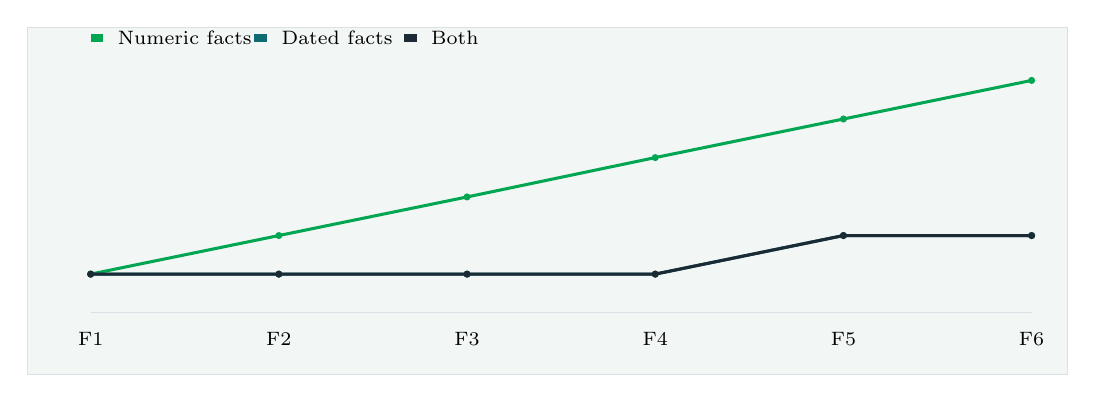
\begin{tikzpicture}[x=1cm,y=1cm]
\path[use as bounding box] (0,0) rectangle (13.20,4.40);
\fill[BOLight] (0,0) rectangle (13.20,4.40);
\draw[BOLine,line width=.35pt] (0,0) rectangle (13.20,4.40);
\draw[BOLine] (0.80,0.78) -- (12.75,0.78);
\draw[BOGreen,line width=1.1pt] (0.80,1.27) -- (3.19,1.76) -- (5.58,2.25) -- (7.97,2.75) -- (10.36,3.24) -- (12.75,3.73);
\fill[BOGreen] (0.80,1.27) circle (.045);
\fill[BOGreen] (3.19,1.76) circle (.045);
\fill[BOGreen] (5.58,2.25) circle (.045);
\fill[BOGreen] (7.97,2.75) circle (.045);
\fill[BOGreen] (10.36,3.24) circle (.045);
\fill[BOGreen] (12.75,3.73) circle (.045);
\draw[BOBlue,line width=1.1pt] (0.80,1.27) -- (3.19,1.27) -- (5.58,1.27) -- (7.97,1.27) -- (10.36,1.76) -- (12.75,1.76);
\fill[BOBlue] (0.80,1.27) circle (.045);
\fill[BOBlue] (3.19,1.27) circle (.045);
\fill[BOBlue] (5.58,1.27) circle (.045);
\fill[BOBlue] (7.97,1.27) circle (.045);
\fill[BOBlue] (10.36,1.76) circle (.045);
\fill[BOBlue] (12.75,1.76) circle (.045);
\draw[BONavy,line width=1.1pt] (0.80,1.27) -- (3.19,1.27) -- (5.58,1.27) -- (7.97,1.27) -- (10.36,1.76) -- (12.75,1.76);
\fill[BONavy] (0.80,1.27) circle (.045);
\fill[BONavy] (3.19,1.27) circle (.045);
\fill[BONavy] (5.58,1.27) circle (.045);
\fill[BONavy] (7.97,1.27) circle (.045);
\fill[BONavy] (10.36,1.76) circle (.045);
\fill[BONavy] (12.75,1.76) circle (.045);
\node[anchor=north,align=center,text width=1.8cm] at (0.80,0.66) {\scriptsize F1};
\node[anchor=north,align=center,text width=1.8cm] at (3.19,0.66) {\scriptsize F2};
\node[anchor=north,align=center,text width=1.8cm] at (5.58,0.66) {\scriptsize F3};
\node[anchor=north,align=center,text width=1.8cm] at (7.97,0.66) {\scriptsize F4};
\node[anchor=north,align=center,text width=1.8cm] at (10.36,0.66) {\scriptsize F5};
\node[anchor=north,align=center,text width=1.8cm] at (12.75,0.66) {\scriptsize F6};
\fill[BOGreen] (0.80,4.22) rectangle (0.96,4.32);
\node[anchor=west] at (1.02,4.27) {\scriptsize Numeric facts};
\fill[BOBlue] (2.88,4.22) rectangle (3.04,4.32);
\node[anchor=west] at (3.10,4.27) {\scriptsize Dated facts};
\fill[BONavy] (4.78,4.22) rectangle (4.94,4.32);
\node[anchor=west] at (5.00,4.27) {\scriptsize Both};
\end{tikzpicture}\par\vspace{2pt}
\vspace{1pt}\noindent\begin{minipage}[t]{0.56\linewidth}
{\footnotesize\color{BOText} Facts that combine dates and numbers are easier for a board reader to verify and compare across sources.}\par
\end{minipage}\hfill\begin{minipage}[t]{0.36\linewidth}
{\scriptsize\color{BOText}\begin{tabular}{p{31mm}>{\raggedleft\arraybackslash}p{18mm}}
\multicolumn{2}{l}{\textcolor{BOGreen}{\bfseries Visible readout}}\\[2pt]
F1 & \textbf{3}\\[1pt]
F2 & \textbf{4}\\[1pt]
F3 & \textbf{5}\\[1pt]
F4 & \textbf{6}\\[1pt]
F5 & \textbf{9}\\[1pt]
\end{tabular}}\par
\end{minipage}\par\vspace{1pt}
\vspace{4pt}{\footnotesize\color{BOText} Facts that combine dates and numbers are easier for a board reader to verify and compare across sources.}\par
{\scriptsize\color{BOMuted} Sources: science.osti.gov; energy.gov; iaea.org; iter.org.}\par

\clearpage
\label{chap:7}
\noindent\begin{tikzpicture}
\path[use as bounding box] (0,0) rectangle (\linewidth,54mm);
\clip (0,0) rectangle (\linewidth,54mm);
\node[anchor=north west,inner sep=0] at (0,54mm) {
\includegraphics[width=\linewidth]{assets/image-7.png}};
\end{tikzpicture}
\vspace{0pt}
\noindent
\begin{tikzpicture}
\fill[BOGreen] (0,0) rectangle (96mm,1.2pt);
\end{tikzpicture}\par\vspace{8pt}
{\Large\sffamily\bfseries\color{BONavy} Regulation, policy and public acceptance can reset the speed of adoption}\par\vspace{4pt}
{\sffamily\fontsize{15}{20}\selectfont\color{BOGreen} External rules can accelerate the market or change the risk budget and project timeline.}\par\vspace{9pt}
\begin{multicols}{2}
{\small Policy support, permitting rules, standards and public acceptance affect how quickly an opportunity moves from concept to deployment. These factors are part of the investment case, not background context.}\par
{\small Where the regulatory path is unclear, the better move is usually standards engagement, policy tracking and low-risk pilots rather than an early heavy-asset commitment.}\par
{\small The board should track which policy events would change investment timing, such as licensing rules, procurement requirements, subsidy treatment, local approvals or safety standards.}\par
{\small From a customer lens, the executive question around Regulation, policy and public acceptance can reset the speed of adoption is practical: which commitments create learning without locking the company into a cost curve, customer promise or regulatory position that the facts cannot yet support.}\par
{\small Capital tied to Regulation, policy and public acceptance can reset the speed of adoption should move only when proof improves along the dimensions that change a business case: customer demand, cost position, financing availability, regulatory path and delivery capability. If those facts do not improve, larger exposure creates lock-in rather than conviction.}\par
{\small For policy exposure, the strongest public fact pattern for Regulation, policy and public acceptance can reset the speed of adoption is narrow but useful: The Department of Energy has been a leader in fusion energy research since the 1950s and supports groundbreaking advances today. It should shape the next customer, cost or partner question without being stretched into proof of commercial scale.}\par
\end{multicols}
\label{chap:7:end}

\clearpage
\label{chap:8}
\noindent\begin{tikzpicture}
\path[use as bounding box] (0,0) rectangle (\linewidth,54mm);
\clip (0,0) rectangle (\linewidth,54mm);
\node[anchor=north west,inner sep=0] at (0,54mm) {
\includegraphics[width=\linewidth]{assets/image-8.png}};
\end{tikzpicture}
\vspace{0pt}
\noindent
\begin{tikzpicture}
\fill[BOGreen] (0,0) rectangle (96mm,1.2pt);
\end{tikzpicture}\par\vspace{8pt}
{\Large\sffamily\bfseries\color{BONavy} Supply chain, partners and talent will decide who can act before the market is obvious}\par\vspace{4pt}
{\sffamily\fontsize{15}{20}\selectfont\color{BOGreen} Strategic advantage comes from ecosystem position rather than standalone product capability.}\par\vspace{9pt}
\begin{multicols}{2}
{\small In uncertain markets, early advantage often comes from supply access, partner entry, talent pools and customer learning rather than a single technology claim.}\par
{\small Management should identify which capabilities are scarce and can be secured early: critical supply, engineering delivery, channel partners, service network, financing partners and compliance capacity. Low-cost learning rights can be more valuable than waiting for full market clarity.}\par
{\small Partnerships should create observable proof points. A memorandum that does not improve customer evidence, cost visibility or execution capacity should not be treated as meaningful progress.}\par
{\small For resource allocation, the executive question around Supply chain, partners and talent will decide who can act before the market is obvious is practical: which commitments create learning without locking the company into a cost curve, customer promise or regulatory position that the facts cannot yet support.}\par
{\small Capital tied to Supply chain, partners and talent will decide who can act before the market is obvious should move only when proof improves along the dimensions that change a business case: customer demand, cost position, financing availability, regulatory path and delivery capability. If those facts do not improve, larger exposure creates lock-in rather than conviction.}\par
{\small From a delivery lens, the strongest public fact pattern for Supply chain, partners and talent will decide who can act before the market is obvious is narrow but useful: The Department of Energy has been a leader in fusion energy research since the 1950s and supports groundbreaking advances today. It should shape the next customer, cost or partner question without being stretched into proof of commercial scale.}\par
\end{multicols}
\label{chap:8:end}

\clearpage
{\textcolor{BOGreen}{\scriptsize\bfseries EXHIBIT 13}}\par\vspace{4pt}
{\sffamily\fontsize{17}{21}\selectfont\color{BONavy} Strategic coverage balances market, cost, policy and execution proof}\par
{\small\color{BOText} Relative coverage on a five-point scale.}\par\vspace{6pt}
\noindent\fcolorbox{BOLine}{BOLight}{\begin{minipage}{0.96\linewidth}\vspace{4pt}{\scriptsize\begin{tabular}{p{38mm}>{\centering\arraybackslash}p{21mm}>{\centering\arraybackslash}p{21mm}>{\centering\arraybackslash}p{21mm}>{\centering\arraybackslash}p{21mm}}
 & {\bfseries Market} & {\bfseries Cost} & {\bfseries Policy} & {\bfseries Execution} \\
\hline
{\bfseries Fusion Commercialization Is} & \colorbox{BOGreen}{\textcolor{white}{\strut\hspace{5pt}5\hspace{5pt}}} & \colorbox{BOGreen}{\textcolor{white}{\strut\hspace{5pt}4\hspace{5pt}}} & \colorbox{BOBlue}{\textcolor{white}{\strut\hspace{5pt}3\hspace{5pt}}} & \colorbox{BOGreen}{\textcolor{white}{\strut\hspace{5pt}5\hspace{5pt}}} \\
{\bfseries Technology Progress Is} & \colorbox{BOGreen}{\textcolor{white}{\strut\hspace{5pt}5\hspace{5pt}}} & \colorbox{BOBlue}{\textcolor{white}{\strut\hspace{5pt}3\hspace{5pt}}} & \colorbox{BOLight}{\textcolor{BOText}{\strut\hspace{5pt}1\hspace{5pt}}} & \colorbox{BOGreen}{\textcolor{white}{\strut\hspace{5pt}5\hspace{5pt}}} \\
{\bfseries Fusion Will Initially Be} & \colorbox{BOGreen}{\textcolor{white}{\strut\hspace{5pt}5\hspace{5pt}}} & \colorbox{BOGreen}{\textcolor{white}{\strut\hspace{5pt}5\hspace{5pt}}} & \colorbox{BOLight}{\textcolor{BOText}{\strut\hspace{5pt}1\hspace{5pt}}} & \colorbox{BOGreen}{\textcolor{white}{\strut\hspace{5pt}5\hspace{5pt}}} \\
{\bfseries Nuclear Fusion} & \colorbox{BOGreen}{\textcolor{white}{\strut\hspace{5pt}5\hspace{5pt}}} & \colorbox{BOGreen}{\textcolor{white}{\strut\hspace{5pt}5\hspace{5pt}}} & \colorbox{BOLight}{\textcolor{BOText}{\strut\hspace{5pt}2\hspace{5pt}}} & \colorbox{BOGreen}{\textcolor{white}{\strut\hspace{5pt}5\hspace{5pt}}} \\
{\bfseries Commercial readiness depends on} & \colorbox{BOGreen}{\textcolor{white}{\strut\hspace{5pt}5\hspace{5pt}}} & \colorbox{BOGreen}{\textcolor{white}{\strut\hspace{5pt}5\hspace{5pt}}} & \colorbox{BOLight}{\textcolor{BOText}{\strut\hspace{5pt}1\hspace{5pt}}} & \colorbox{BOGreen}{\textcolor{white}{\strut\hspace{5pt}5\hspace{5pt}}} \\
\end{tabular}}\vspace{4pt}\end{minipage}}\par\vspace{2pt}
\vspace{1pt}\noindent\begin{minipage}[t]{0.56\linewidth}
{\footnotesize\color{BOText} A balanced executive view connects the market case with cost evidence, policy timing and execution constraints.}\par
\end{minipage}\hfill\begin{minipage}[t]{0.36\linewidth}
{\scriptsize\color{BOText}\begin{tabular}{p{31mm}>{\raggedleft\arraybackslash}p{18mm}}
\multicolumn{2}{l}{\textcolor{BOGreen}{\bfseries Matrix readout}}\\[2pt]
Fusion & \textbf{5 / 4}\\[1pt]
Technology Progress & \textbf{5 / 3}\\[1pt]
Fusion Will Initially & \textbf{5 / 5}\\[1pt]
Nuclear Fusion & \textbf{5 / 5}\\[1pt]
\end{tabular}}\par
\end{minipage}\par\vspace{1pt}
\vspace{4pt}{\footnotesize\color{BOText} A balanced executive view connects the market case with cost evidence, policy timing and execution constraints.}\par
{\scriptsize\color{BOMuted} Sources: public references and report analysis.}\par
\vspace{9pt}\textcolor{BOLine}{\rule{\linewidth}{0.3pt}}\vspace{8pt}
{\textcolor{BOGreen}{\scriptsize\bfseries EXHIBIT 14}}\par\vspace{4pt}
{\sffamily\fontsize{17}{21}\selectfont\color{BONavy} Triangulation is strongest where domains, facts and years overlap}\par
{\small\color{BOText} Composite view of public domains, extracted facts and explicit dates.}\par\vspace{6pt}
\noindent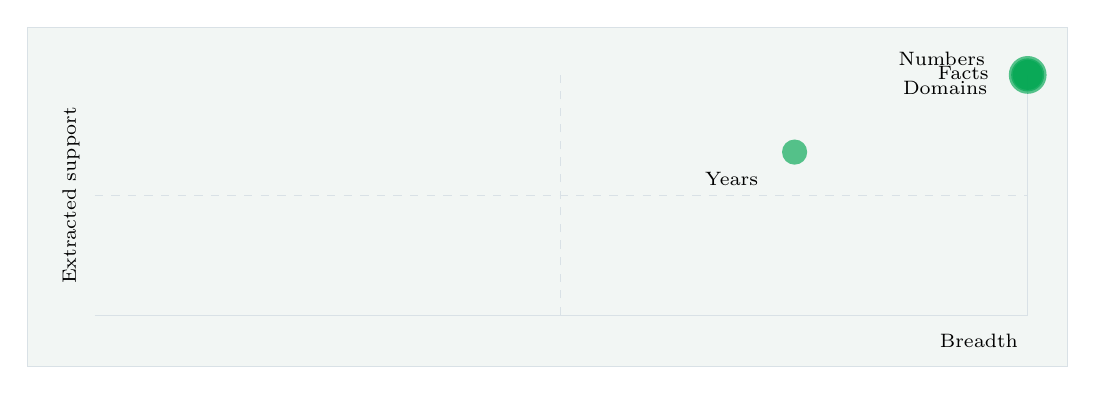
\begin{tikzpicture}[x=1cm,y=1cm]
\path[use as bounding box] (0,0) rectangle (13.20,4.30);
\fill[BOLight] (0,0) rectangle (13.20,4.30);
\draw[BOLine,line width=.35pt] (0,0) rectangle (13.20,4.30);
\draw[BOLine] (0.85,0.65) -- (12.70,0.65) -- (12.70,3.70);
\draw[BOLine,dashed] (0.85,2.17) -- (12.70,2.17);
\draw[BOLine,dashed] (6.77,0.65) -- (6.77,3.70);
\fill[BOGreen,opacity=.65] (12.70,3.70) circle (0.21);
\node[anchor=east,align=right,text width=2.10cm] at (12.31,3.54) {\scriptsize Domains};
\fill[BOGreen,opacity=.65] (12.70,3.70) circle (0.19);
\node[anchor=east,align=right,text width=2.10cm] at (12.33,3.73) {\scriptsize Facts};
\fill[BOGreen,opacity=.65] (9.74,2.72) circle (0.16);
\node[anchor=east,align=right,text width=2.10cm] at (9.40,2.38) {\scriptsize Years};
\fill[BOGreen,opacity=.65] (12.70,3.70) circle (0.24);
\node[anchor=east,align=right,text width=2.10cm] at (12.28,3.91) {\scriptsize Numbers};
\node[anchor=north east] at (12.70,0.53) {\scriptsize Breadth};
\node[anchor=center,rotate=90] at (0.55,2.17) {\scriptsize Extracted support};
\end{tikzpicture}\par\vspace{2pt}
\vspace{1pt}\noindent\begin{minipage}[t]{0.56\linewidth}
{\footnotesize\color{BOText} The commercial conclusion becomes more credible when multiple source domains, fact types and dated milestones point in the same direction.}\par
\end{minipage}\hfill\begin{minipage}[t]{0.36\linewidth}
{\scriptsize\color{BOText}\begin{tabular}{p{31mm}>{\raggedleft\arraybackslash}p{18mm}}
\multicolumn{2}{l}{\textcolor{BOGreen}{\bfseries Position}}\\[2pt]
Domains & \textbf{100 / 100}\\[1pt]
Facts & \textbf{100 / 100}\\[1pt]
Years & \textbf{75 / 68}\\[1pt]
Numbers & \textbf{100 / 100}\\[1pt]
\end{tabular}}\par
\end{minipage}\par\vspace{1pt}
\vspace{4pt}{\footnotesize\color{BOText} The commercial conclusion becomes more credible when multiple source domains, fact types and dated milestones point in the same direction.}\par
{\scriptsize\color{BOMuted} Sources: science.osti.gov; energy.gov; iaea.org; iter.org.}\par

\clearpage
\noindent
\begin{tikzpicture}
\fill[BOGreen] (0,0) rectangle (46mm,1.2pt);
\end{tikzpicture}\par\vspace{8pt}
{\sffamily\fontsize{22}{27}\selectfont\color{BONavy} Research basis and limitations}\par\vspace{9pt}
\begin{minipage}[t]{0.47\linewidth}
{\sffamily\fontsize{15}{20}\selectfont\color{BOGreen} Public materials support a strategic view, not a transaction recommendation.}\par\vspace{7pt}
{\footnotesize\color{BOText} This report has been prepared for strategy discussion and executive decision support. It is not investment, legal, tax, audit or valuation advice. Market estimates, forecasts and scenarios are directional and should be independently validated before they are used for investment, financing, transaction, regulatory or operational decisions. Forward-looking views may change as technology, policy, financing, regulation, competition, supply chains and macro conditions evolve. Recipients should perform their own diligence and treat this report as one input into a broader decision process.}\par
\end{minipage}\hfill\begin{minipage}[t]{0.46\linewidth}
{\textcolor{BOGreen}{\scriptsize\bfseries PUBLIC MATERIALS REFERENCED}}\par\vspace{5pt}
\begin{tabularx}{\linewidth}{p{8mm}Y}
\textcolor{BOGreen}{\bfseries 01} & {\scriptsize Osti} \\[4pt]
\textcolor{BOGreen}{\bfseries 02} & {\scriptsize Energy} \\[4pt]
\textcolor{BOGreen}{\bfseries 03} & {\scriptsize Iaea} \\[4pt]
\textcolor{BOGreen}{\bfseries 04} & {\scriptsize Iter} \\[4pt]
\textcolor{BOGreen}{\bfseries 05} & {\scriptsize Nationalacademies} \\[4pt]
\textcolor{BOGreen}{\bfseries 06} & {\scriptsize Fusionindustryassociation} \\[4pt]
\textcolor{BOGreen}{\bfseries 07} & {\scriptsize Llnl} \\[4pt]
\end{tabularx}
\end{minipage}\par\vspace{12pt}
\fcolorbox{BOLine}{BOLight}{\begin{minipage}{0.96\linewidth}\vspace{5pt}\begin{tabularx}{\linewidth}{Y Y Y}
{\textcolor{BOGreen}{\scriptsize\bfseries USE}}\par{\scriptsize Use the report to clarify timing, partner selection, capital exposure and the next management decision.} & {\textcolor{BOGreen}{\scriptsize\bfseries DO NOT USE}}\par{\scriptsize Do not treat directional market views as a substitute for transaction diligence, technical verification or legal advice.} & {\textcolor{BOGreen}{\scriptsize\bfseries UPDATE TRIGGER}}\par{\scriptsize Refresh the view when public milestones, cost curves, regulation, financing or customer commitments materially change.} \\
\end{tabularx}\vspace{5pt}\end{minipage}}

\clearpage
\noindent
\begin{tikzpicture}
\fill[BOGreen] (0,0) rectangle (38mm,1.2pt);
\end{tikzpicture}\par\vspace{8pt}
{\sffamily\fontsize{24}{30}\selectfont\color{BONavy} About BlueOcean}\par\vspace{10pt}
\begin{minipage}[t]{0.44\linewidth}
{\sffamily\fontsize{16}{22}\selectfont\color{BOGreen} Research is most useful when it changes a management decision.}\par\vspace{8pt}
{\footnotesize\color{BOText} BlueOcean prepares decision-focused research for executives who need to separate credible evidence from market noise, translate technology shifts into commercial implications and stage commitments around proof.}\par\vspace{7pt}
{\footnotesize\color{BOMuted} This report draws on Osti, Energy, Iaea, Iter, Nationalacademies, Fusionindustryassociation, Llnl.}\par
\vspace{10pt}\fcolorbox{BOLine}{BOLight}{\begin{minipage}{0.90\linewidth}\vspace{5pt}{\scriptsize\color{BOText} The work is designed for CEOs and leadership teams who need a concise view of what changes now, what waits for stronger proof and which external facts would change the answer.}\vspace{5pt}\end{minipage}}
\end{minipage}\hfill\begin{minipage}[t]{0.48\linewidth}
{\textcolor{BOGreen}{\scriptsize\bfseries HOW BLUEOCEAN SUPPORTS EXECUTIVE TEAMS}}\par\vspace{5pt}
\begin{tabularx}{\linewidth}{p{8mm}Y}
\textcolor{BOGreen}{\bfseries 01} & {\scriptsize\bfseries Strategy research}\par{\scriptsize Decision-focused market, technology and competitive research for senior leadership.} \\[6pt]
\textcolor{BOGreen}{\bfseries 02} & {\scriptsize\bfseries Evidence synthesis}\par{\scriptsize Structured comparison of public materials, company claims, policy signals and market data.} \\[6pt]
\textcolor{BOGreen}{\bfseries 03} & {\scriptsize\bfseries Executive output}\par{\scriptsize Reader-ready reports, exhibits and board materials designed for fast management discussion.} \\[6pt]
\textcolor{BOGreen}{\bfseries 04} & {\scriptsize\bfseries Quality control}\par{\scriptsize Source retention, language cleanup and layout checks before publication.} \\[6pt]
\end{tabularx}\vspace{6pt}
\begin{tabularx}{\linewidth}{p{31mm}Y}
{\small\bfseries This report was prepared by the Energy Strategy Practice of a global management}\par{\scriptsize\color{BOGreen} Research synthesis team} & {\footnotesize Responsible for evidence checks, executive synthesis and report QA.} \\[7pt]
{\small\bfseries The analysis was reviewed by a panel of fusion physicists and energy economists}\par{\scriptsize\color{BOGreen} Research synthesis team} & {\footnotesize Responsible for evidence checks, executive synthesis and report QA.} \\[7pt]
{\small\bfseries The report team has advised Fortune 500 energy companies and government}\par{\scriptsize\color{BOGreen} Research synthesis team} & {\footnotesize Responsible for evidence checks, executive synthesis and report QA.} \\[7pt]
\end{tabularx}
\end{minipage}

\clearpage
\thispagestyle{empty}
\AddToShipoutPictureBG*{\AtPageLowerLeft{
\includegraphics[width=\paperwidth,height=\paperheight]{assets/cover-ai.png}}}

\vspace*{\fill}
\begin{flushright}
{\sffamily\bfseries\Large\color{white} BlueOcean}\hspace*{3mm}
\end{flushright}
\vspace*{8mm}

\end{document}
